\documentclass[12pt,a4paper]{article}

% ── Packages ──────────────────────────────────────────────────────────────
\usepackage[utf8]{inputenc}
\usepackage[T1]{fontenc}
\usepackage{geometry}
% 178 mm text block so the 178 mm-wide figure sources print at 1:1 (7 pt labels),
% instead of 0.95 x 160 mm = 152 mm, which shrank them to ~6 pt.
\geometry{left=16mm,right=16mm,top=22mm,bottom=18mm,headheight=13pt,headsep=5mm,footskip=8mm}
\usepackage{graphicx}
\usepackage{amsmath}
\usepackage{lmodern}
\usepackage{microtype}
\usepackage{booktabs}
\usepackage{tabularx}
\usepackage{array}
\usepackage{longtable}
\usepackage{hyperref}
\hypersetup{colorlinks=true, linkcolor=blue, citecolor=blue, urlcolor=blue}
\usepackage{xcolor}
\usepackage{fancyhdr}
\usepackage{float}
\usepackage{needspace}
\usepackage{caption}
\captionsetup{font=small,labelfont=bf}

% Supplementary items carry their own S numbering: the figure environment
% numbers them S1..S13, so captions must not repeat "Figure Sx." by hand.
\renewcommand{\thefigure}{S\arabic{figure}}

% ── Page style ────────────────────────────────────────────────────────────
\pagestyle{fancy}
\fancyhf{}
\fancyhead[L]{\small Supplementary Information}
\fancyhead[R]{\small\textit{Annotation accuracy and differentiation order}}
\fancyfoot[C]{\thepage}
\renewcommand{\headrulewidth}{0.4pt}
\renewcommand{\footrulewidth}{0.4pt}

% Allow long typewriter paths to break (avoid overfull boxes)
\sloppy
\emergencystretch=5em
\raggedbottom

% ── Path to figures (relative from this tex file) ────────────────────────
\graphicspath{{../../../../figures/paper1/}}

% ==========================================================================
\begin{document}

% ── Cover page ────────────────────────────────────────────────────────────
\thispagestyle{empty}
\begin{center}
  \vspace*{3cm}
  {\LARGE\bfseries Supplementary Information}\\[1.5cm]
  {\Large\bfseries Annotation accuracy is not a proxy for differentiation\\[4pt]
   order in fine-tuned single-cell foundation models}\\[1.5cm]
  {\large Kunhui Xu, Chenchen Wang, Fenfen Li, Xiaoyu Chen, Xinyu Wang, Yi Zhang,\\
   Tiancheng Pu, Jiahao Tang, Hongguang Cui, Peng Guo, and Qi Dai}\\[0.5cm]
  {\large $^{1}$The First Affiliated Hospital, Zhejiang University School of Medicine,\\
   Hangzhou, Zhejiang Province 311121, PR China;\\
   $^{2}$Eye Research Center, Hangzhou Institute of Medicine, Chinese Academy of Sciences,\\
   Eye Hospital, Wenzhou Medical University, Hangzhou, Zhejiang Province 310018, PR China}\\[0.5cm]
  {\large Hongguang Cui (\texttt{1189002@zju.edu.cn}), Peng Guo (\texttt{guopeng@ucas.ac.cn}), and\\
   Qi Dai (\texttt{dq@mail.eye.ac.cn}) --- corresponding authors}\\[1.5cm]
  {\large Compiled \today}\\[2cm]
  \end{center}
\newpage

% ── Table of Contents (manual, using \pageref) ────────────────────────────
\section*{Contents}
\addcontentsline{toc}{section}{Contents}

\paragraph*{Supplementary Figures}
\begin{description}
  \item[Figure S1]\hfill\pageref{fig:S1} -- Per-class reliability diagrams
  \item[Figure S2]\hfill\pageref{fig:S2} -- Out-of-distribution confidence analysis
  \item[Figure S3]\hfill\pageref{fig:S3} -- Per-seed reproducibility
  \item[Figure S4]\hfill\pageref{fig:S4} -- Quality control of GSE153515
  \item[Figure S5]\hfill\pageref{fig:S5} -- Training dynamics
  \item[Figure S6]\hfill\pageref{fig:S6} -- Per-donor macro-F1 breakdown
  \item[Figure S7]\hfill\pageref{fig:S7} -- Layer-resolved $\rho$ per seed
  \item[Figure S8]\hfill\pageref{fig:S8} -- External test annotation detail
  \item[Figure S9]\hfill\pageref{fig:S9} -- TAC sensitivity analysis
  \item[Figure S10]\hfill\pageref{fig:S10} -- Ordinal head decision boundaries
  \item[Figure S11]\hfill\pageref{fig:S11} -- Trajectory inference
  \item[Figure S12]\hfill\pageref{fig:S12} -- Annotation of external test sets
  \item[Figure S13]\hfill\pageref{fig:S13} -- Continuity metrics under task adaptation
\end{description}

\paragraph*{Supplementary Tables}
\begin{description}
  \item[Table S1]\hfill\pageref{tab:S1} -- Primary external-test metrics (per-seed, per-donor, per-class)
  \item[Table S2]\hfill\pageref{tab:S2} -- Label-set and step-budget controls
  \item[Table S3]\hfill\pageref{tab:S3} -- Layer-resolved $\rho$
  \item[Table S4]\hfill\pageref{tab:S4} -- Frozen-representation probes
  \item[Table S5]\hfill\pageref{tab:S5} -- Training-atlas composition and provenance
  \item[Table S6]\hfill\pageref{tab:S6} -- scGPT-human same-corpus arms (per-seed, budgets)
  \item[Table S7]\hfill\pageref{tab:S7} -- scGPT-human convergence checkpoints
  \item[Table S8]\hfill\pageref{tab:S8} -- Geneformer official-budget control
  \item[Table S9]\hfill\pageref{tab:S9} -- CellPLM arms
  \item[Table S10]\hfill\pageref{tab:S10} -- Classical baselines
  \item[Table S11]\hfill\pageref{tab:S11} -- CellPLM training-budget dose response
  \item[Table S12]\hfill\pageref{tab:S12} -- Geometry-preserving recipes (scGPT-human, van Zyl)
\end{description}

\paragraph*{Supplementary Data}
\begin{description}
  \item[Data S1--S3]\hfill\pageref{sec:data} -- Raw data descriptions
\end{description}

\paragraph*{Supplementary Methods}
\begin{description}
  \item[Supplementary Methods]\hfill\pageref{sec:suppmethods} -- Configuration, provenance and software details
\end{description}

\newpage

% ==========================================================================
%  Supplementary Figures
% ==========================================================================
\section*{Supplementary Figures}

% ── Figure S1 ─────────────────────────────────────────────────────────────
\begin{figure}[htbp]
  \centering
  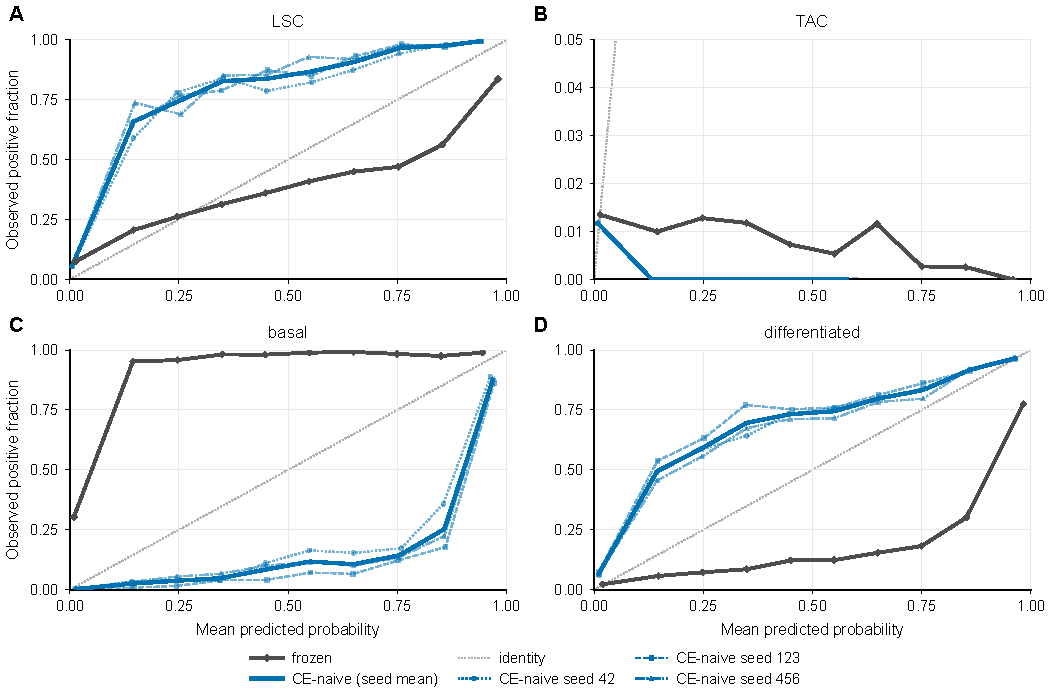
\includegraphics[width=\textwidth]{figureS1_calibration}
  \caption{Per-class reliability diagrams on the external test set (GSE153515). (A--D) One-vs-rest reliability diagrams for the (A) LSC, (B) TAC, (C) basal and (D) differentiated classes, over the 14,775 external epithelial cells of two donors. For each of the four models (frozen Geneformer-V2-104M and CE-naive $\lambda$ = 0; seeds 42, 123 and 456 for the fine-tuned arm; thin lines are individual seeds and the heavy line their three-seed mean), predicted class probabilities were binned into 10 equal-width half-open probability bins \texttt{[lo, hi)} (final bin closed at 1.0), so each cell contributes to exactly one bin; each point plots the mean predicted probability (x-axis) against the observed fraction of class-positive cells (y-axis) for non-empty bins. The TAC class holds 171 true cells (1.2\%) and its panel's y-range is set to its own data (0--0.05), because all posteriors there are near zero. Dotted diagonal: identity (perfect calibration). Reported in Methods, Evaluation metrics. Files: \texttt{figures/paper1/figureS1\_calibration.\{pdf,png\}}; plotted values in \texttt{figureS1\_calibration.csv}. Generated by \texttt{scripts/measure\_percell\_probs.py}.}
  \label{fig:S1}
\end{figure}

% ── Figure S2 ─────────────────────────────────────────────────────────────
\begin{figure}[htbp]
  \centering
  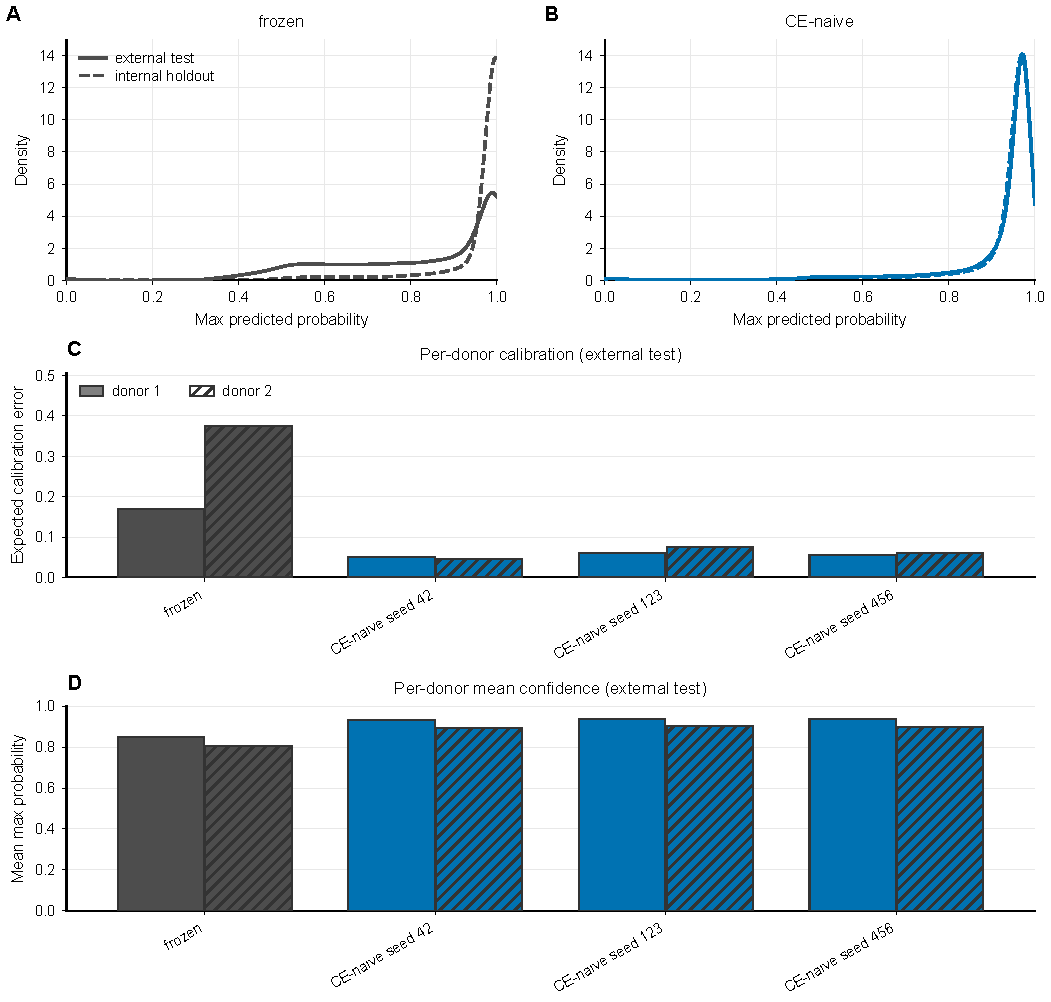
\includegraphics[width=\textwidth]{figureS2_ood}
  \caption{Out-of-distribution confidence analysis. (A--B) Kernel density estimates of the per-cell maximum predicted probability, compared between the external test set (GSE153515) and the internal holdout split, for (A) frozen Geneformer and (B) CE-naive $\lambda$ = 0 (its three seeds pooled); the two panels share one y-limit. (C) Per-donor expected calibration error (ECE) on the external set for all four models, with donor identity encoded by fill within each arm's hue (donor 1 solid, donor 2 hatch-filled). (D) Per-donor mean maximum predicted probability (confidence) on the external set. donor\_1/donor\_2 correspond to GSM4646295/GSM4646296 (Methods, External test annotation pipeline). Reported in Methods, Ordinal head formulation. Files: \texttt{figures/paper1/figureS2\_ood.\{pdf,png\}}; plotted values in \texttt{figureS2\_ood\_maxprob.csv} and \texttt{figureS2\_ood\_perdonor.csv}. Generated by \texttt{scripts/measure\_percell\_probs.py}.}
  \label{fig:S2}
\end{figure}

% ── Figure S3 ─────────────────────────────────────────────────────────────
\begin{figure}[htbp]
  \centering
  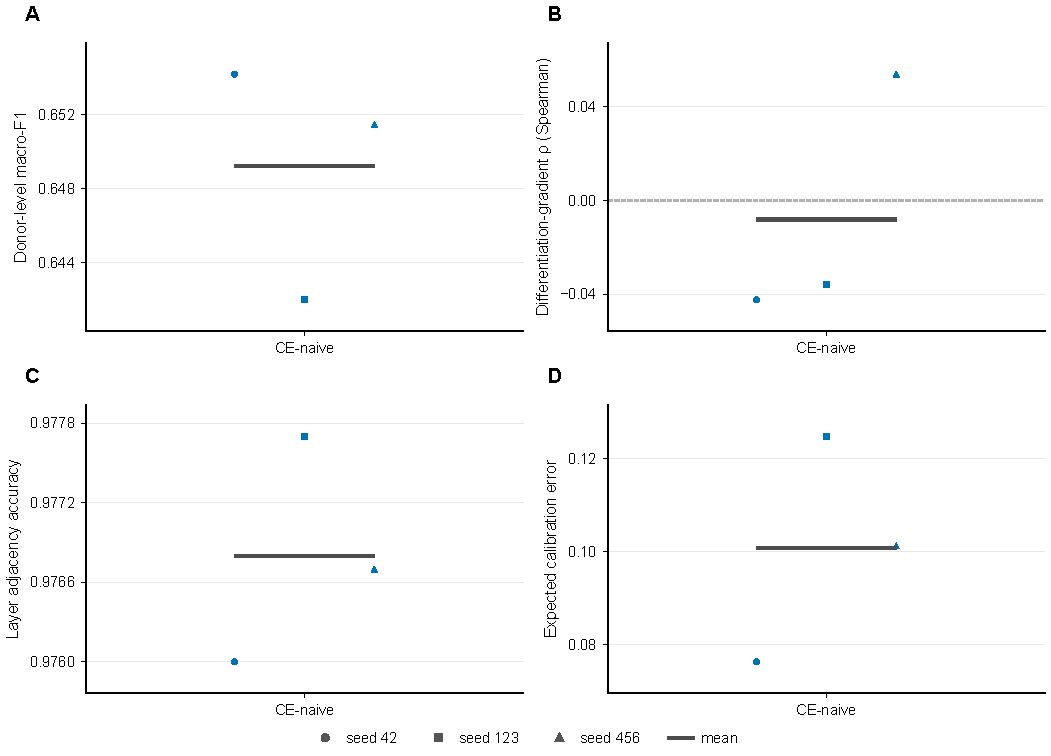
\includegraphics[width=\textwidth]{figureS3_per_seed_reproducibility}
  \caption{Per-seed reproducibility of the endpoint and continuity metrics. Points are individual seeds 42, 123 and 456 (marker shape) for CE-naive ($\lambda$ = 0); the short horizontal tick is the arithmetic mean of the three seeds. (A) Donor-level macro-F1. (B) Differentiation-gradient Spearman $\rho$ between representation-derived cell ordering and prespecified stage ranks; the dotted line marks $\rho$ = 0. (C) Layer adjacency accuracy. (D) Expected calibration error. All values are from the GSE153515 same-corpus external holdout (14,775 epithelial cells, two donors); donor-level macro-F1 is the mean of the two per-donor scores. No interval, test or correction is shown; three seeds per arm. Values from \texttt{figures/paper1/table\_t7\_seed\_reproducibility.csv}; plotted values in \texttt{figureS3\_per\_seed\_reproducibility.csv}. Files: \texttt{figures/paper1/figureS3\_per\_seed\_reproducibility.\{pdf,png\}}. Generated by \texttt{scripts/figureS3\_per\_seed\_reproducibility.py}.}
  \label{fig:S3}
\end{figure}

% ── Figure S4 ─────────────────────────────────────────────────────────────
\begin{figure}[htbp]
  \centering
  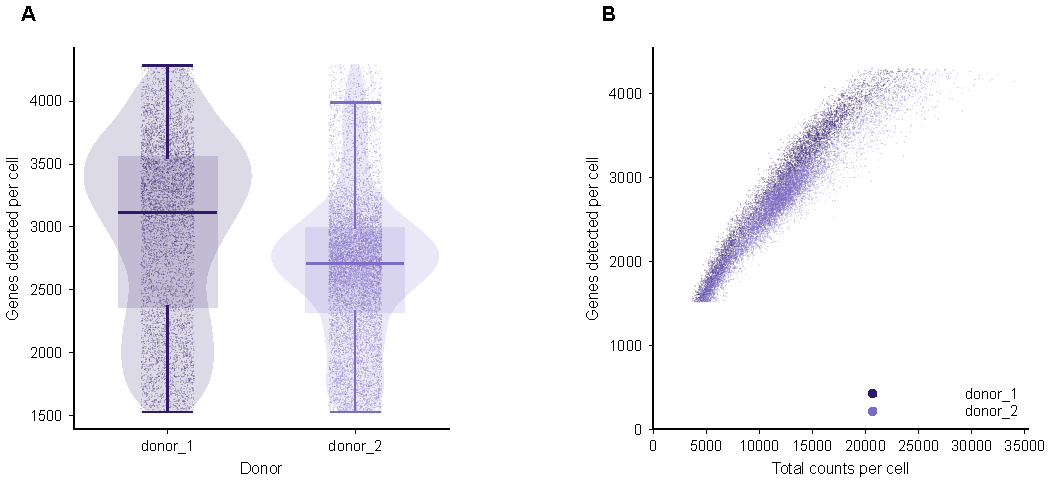
\includegraphics[width=\textwidth]{figureS4_gse153515_qc}
  \caption{Quality control of the external test set (GSE153515). The 15,827 QC-passing cells (10,605 genes) from two donors, annotated per Methods, External test annotation pipeline. (A) Violin plot of genes detected per cell by donor (donor\_1, donor\_2), with box-plot interiors and capped whiskers. (B) Scatter plot of total counts per cell versus genes detected per cell, colored by donor (legend, lower right). No QC cut-off lines are drawn: the locked configuration declares no numeric threshold on genes detected or total counts. Files: \texttt{figures/paper1/figureS4\_gse153515\_qc.\{pdf,png\}}. Generated by \texttt{scripts/figureS4\_gse153515\_qc.py}. Legend consistent with the main results draft.}
  \label{fig:S4}
\end{figure}

% ── Figure S5 ─────────────────────────────────────────────────────────────
\begin{figure}[htbp]
  \centering
  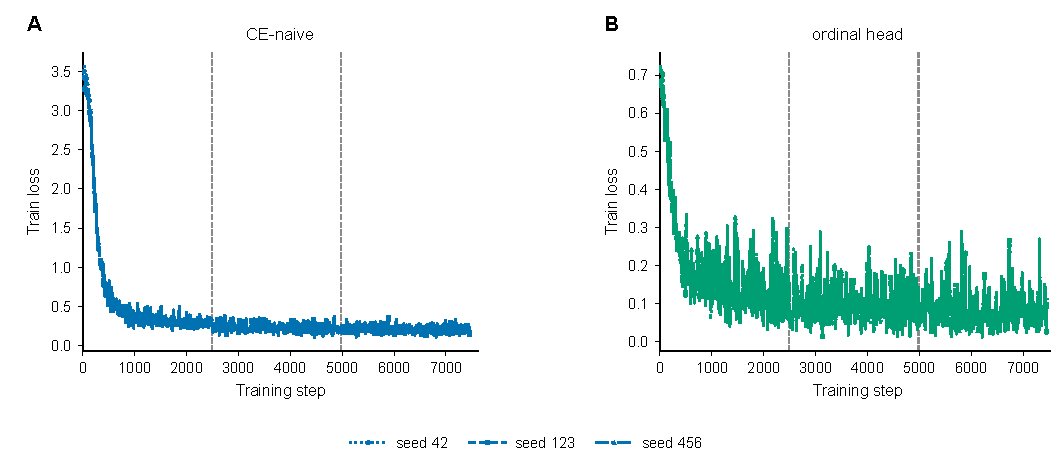
\includegraphics[width=\textwidth]{figureS5_training_dynamics}
  \caption{Training dynamics of the six fine-tuning runs. (A) CE-naive ($\lambda$ = 0; cross-entropy over 31 \texttt{author\_cell\_type} classes). (B) Ordinal head ($\lambda$ = 0; the ordinal cumulative-threshold loss on epithelial cells). Training loss versus training step for each seed (42, 123, 456); three epochs per run, 2,491 steps per epoch and 7,473 steps in total (effective batch size 32). The two arms optimise different objectives over different label spaces, so their loss magnitudes are not comparable: only the trajectory shape, the epoch count and the convergence point can be read across panels, which is why each panel carries its own loss axis. Dashed vertical lines mark the epoch boundaries. Loss records are read directly from \texttt{checkpoint-7473/trainer\_state.json} of the six runs. Files: \texttt{figures/paper1/figureS5\_training\_dynamics.\{pdf,png\}}. Generated by \texttt{scripts/figureS5\_training\_dynamics.py}.}
  \label{fig:S5}
\end{figure}

% ── Figure S6 ─────────────────────────────────────────────────────────────
\begin{figure}[htbp]
  \centering
  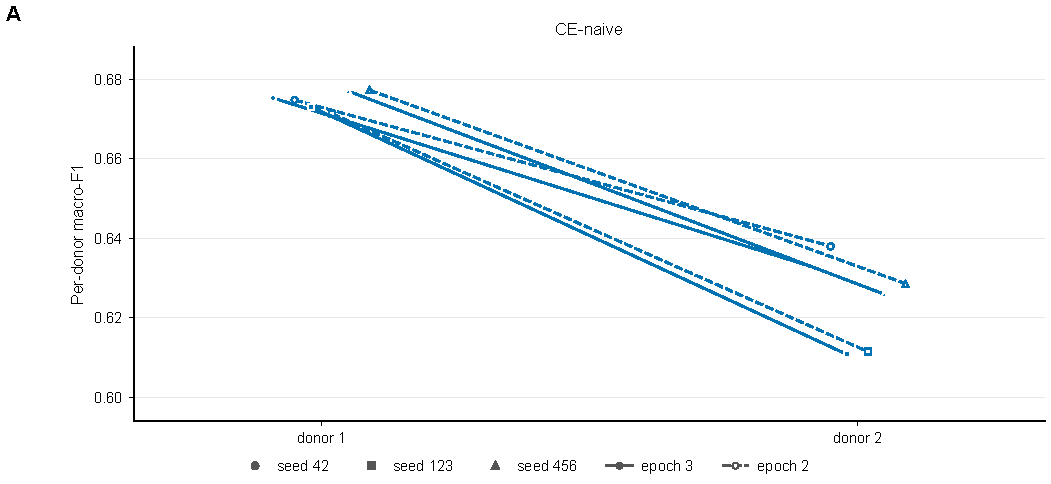
\includegraphics[width=\textwidth]{figureS6_per_donor_breakdown}
  \caption{Per-donor breakdown of the primary endpoint. Lines join the two held-out donors for each seed (marker shape: 42, 123, 456) and epoch (solid, epoch 3; dashed, epoch 2); the single panel shows CE-naive ($\lambda$ = 0). Values are per-donor donor-level macro-F1 (donor\_1 = GSM4646295, donor\_2 = GSM4646296; 14,775 epithelial cells across both donors). All three seeds and both epochs are plotted for both arms; no interval, test or correction is shown. Values from the \texttt{per\_donor} blocks of \texttt{results/paper1\_tier\_b\_eval/results\_\{$\lambda$\}\_\{seed\}.json} and \texttt{results\_epoch2\_\{$\lambda$\}\_\{seed\}.json}; plotted values in \texttt{figureS6\_per\_donor\_breakdown.csv}. See also Table S1. Files: \texttt{figures/paper1/figureS6\_per\_donor\_breakdown.\{pdf,png\}}. Generated by \texttt{scripts/figureS6\_per\_donor\_breakdown.py}.}
  \label{fig:S6}
\end{figure}

% ── Figure S7 ─────────────────────────────────────────────────────────────
\begin{figure}[htbp]
  \centering
  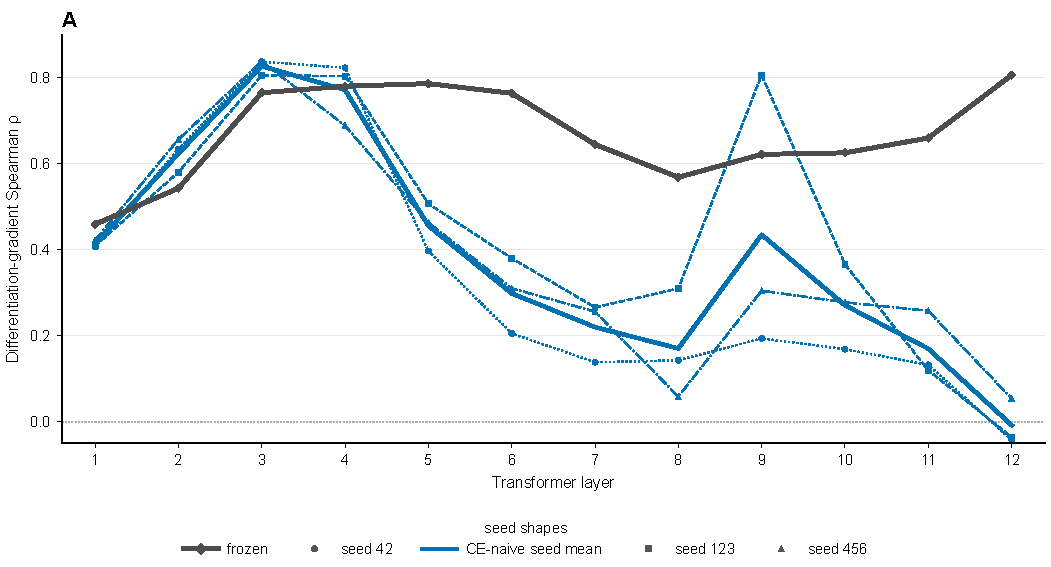
\includegraphics[width=\textwidth]{figureS7_layerwise_rho_per_seed}
  \caption{Layerwise differentiation-gradient Spearman $\rho$ per seed. Hidden states L1--L12 (L0 excluded: constant [CLS]); thin lines are individual seeds (linestyle and marker: 42, 123, 456) and the thick line is the arithmetic mean of the three seeds of that arm. Frozen Geneformer is a single reference run. The external set is GSE153515 (14,775 epithelial cells, two donors). No band, interval, test or correction is shown; three seeds per adapted arm. Layerwise values from \texttt{results/paper1\_layerwise\_rho/layerwise\_rho\_*.json} (see also Table S3); plotted values in \texttt{figureS7\_layerwise\_rho\_per\_seed.csv}. See also Figure 2. Files: \texttt{figures/paper1/figureS7\_layerwise\_rho\_per\_seed.\{pdf,png\}}. Generated by \texttt{scripts/figureS7\_layerwise\_rho\_per\_seed.py}.}
  \label{fig:S7}
\end{figure}

% ── Figure S8 ─────────────────────────────────────────────────────────────
\begin{figure}[htbp]
  \centering
  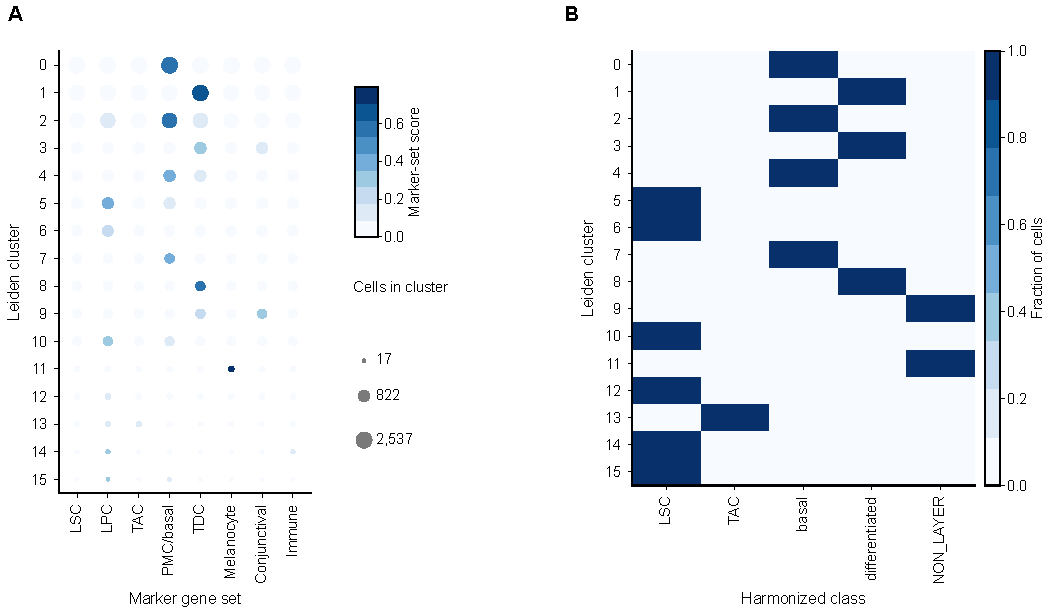
\includegraphics[width=\textwidth]{figureS8_annotation_detail}
  \caption{External test annotation detail (GSE153515). Cluster-level detail of the annotation pipeline for the external-test annotation (Figure S12): (A) cluster-level marker-set scores across the eight curated marker gene sets (colour), with cluster size as dot area; (B) cluster-to-class assignment heatmap for the 16 Leiden clusters, rows sorted numerically. Files: \texttt{figures/paper1/figureS8\_annotation\_detail.\{pdf,png\}}. Generated by \texttt{scripts/figureS8\_annotation\_detail.py}.}
  \label{fig:S8}
\end{figure}

% ── Figure S9 ────────────────────────────────────────────────────────────
\begin{figure}[htbp]
  \centering
  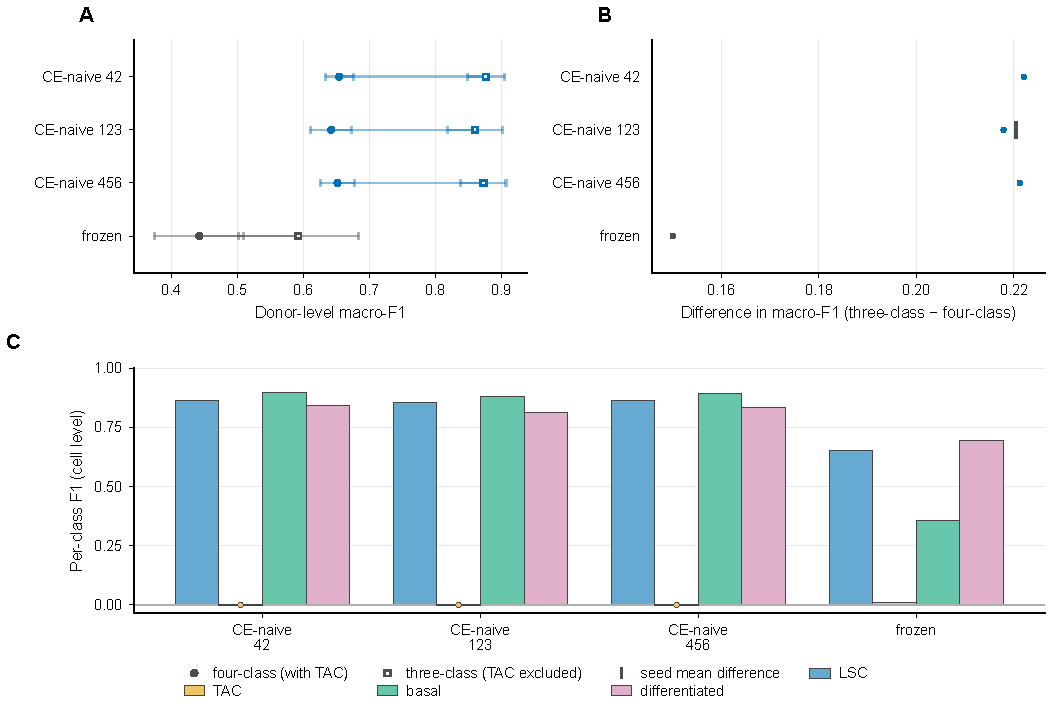
\includegraphics[width=\textwidth]{figureS9_tac_sensitivity}
  \caption{Sensitivity of the primary endpoint to the rare TAC class. (A) Donor-level macro-F1 under the locked four-class schema (filled circles) and the three-class schema with TAC excluded (open squares); horizontal bars are the donor-level bootstrap 95\% CI (1,000 donor resamples, bootstrap seed 42), drawn per run and never pooled. (B) Difference between the two endpoints, computed within each seed (points) and then averaged over the three seeds (tick); no interval is drawn for the difference because the two endpoints were bootstrapped separately. (C) Pooled cell-level per-class F1 under the four-class schema. GSE153515 external test: 14,775 epithelial cells, two donors, 171 TAC cells (1.2\%). CE-naive has three seeds (42, 123, 456); frozen is one reference run. Files: \texttt{figures/paper1/figureS9\_tac\_sensitivity.\{pdf,png\}}. Generated by \texttt{scripts/analyze\_tac\_sensitivity.py}.}
  \label{fig:S9}
\end{figure}

% ── Figure S10 ────────────────────────────────────────────────────────────
\begin{figure}[htbp]
  \centering
  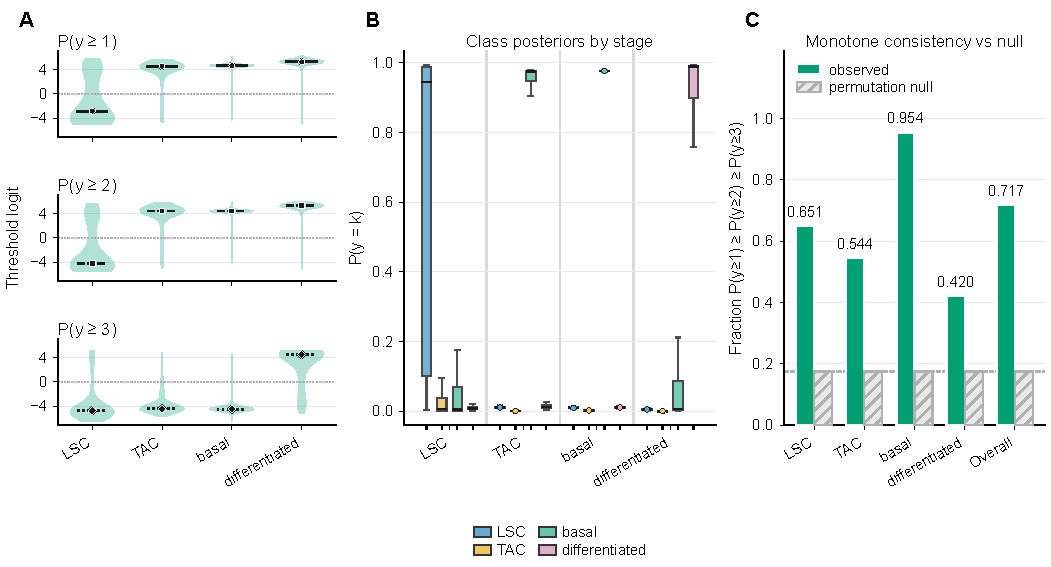
\includegraphics[width=\textwidth]{figureS10_ordinal_boundaries}
  \caption{Ordinal head decision boundaries. Mechanistic evidence that the unconditional cumulative-threshold ordinal head (arm: ordinal head; $\lambda$ = 0; seed 42; terminal checkpoint-7473, epoch 3; unlike a standard conditional cumulative-threshold head, all valid cells contribute to every threshold and the outputs are not constrained to be monotone) learns ordered, monotone decision boundaries rather than an unordered classifier, on the external test set (GSE153515, $n$ = 14,775 epithelial cells). Boxes are median with 1.5$\times$IQR whiskers; outliers are not shown. (A) Distribution of the three threshold logits of the ordinal head ($t_1$--$t_3$; the plotted quantity is the raw threshold logit, not a probability, whereas head $k$ is trained to predict $P(y \ge k)$) by differentiation stage. The thresholds form an ordered cascade along the differentiation axis: $t_1$ and $t_2$ are high for TAC/basal/differentiated and low for LSC (median logits $-$2.86 $\rightarrow$ $+$4.63/$-$4.19 $\rightarrow$ $+$4.41 across LSC $\rightarrow$ basal), whereas $t_3$ is high only for differentiated ($+$4.47 vs $-$4.44 to $-$4.78 elsewhere), so each boundary separates one ordered segment of the axis. (B) Predicted class probabilities $P(y = k) = p_k - p_{k+1}$ by stage: each stage allocates its posterior mass to its own (or an adjacent) class in axis order: LSC cells to $P(\text{LSC})$ (median 0.945), basal to $P(\text{basal})$ (0.976), differentiated to $P(\text{differentiated})$ (0.989), with intermediate classes lying between (TAC cells, $n$ = 171, to the adjacent basal, median 0.975); near-zero posteriors are marked explicitly with open diamonds. (C) Per-cell cumulative-probability monotonic consistency, i.e. the fraction of cells with $P(y \ge 1) \ge P(y \ge 2) \ge P(y \ge 3)$: observed 0.717 overall (seed 42; per stage: LSC 0.651, TAC 0.544, basal 0.954, differentiated 0.420; the lower values on saturated stages reflect all three thresholds near 0 or 1, where small per-cell noise flips the ordering) versus 0.175 expected under an unordered head (criterion: seeded within-cell permutation of the three threshold slots, 1,000 draws, seed 42). Robustness: three-seed (42/123/456) overall consistency 0.7172 / 0.8719 / 0.7877 (mean 0.7923, range 0.7172--0.8719), all far above the permutation null of 0.1751 (1,000 draws, seed 42). Reported in Results (Ordinal supervision and LoRA preserve stage ordering in same-corpus tests). Files: \texttt{figures/paper1/figureS10\_ordinal\_boundaries.\{pdf,png\}}. Generated by \texttt{scripts/figureS10\_ordinal\_boundaries.py} (figure), from per-cell threshold logits and probabilities extracted by \texttt{scripts/extract\_ordinal\_logits.py} (npz/json in \texttt{results/paper1\_corn\_boundary/}).}
  \label{fig:S10}
\end{figure}

% ── Figure S11 ────────────────────────────────────────────────────────────
\begin{figure}[htbp]
  \centering
  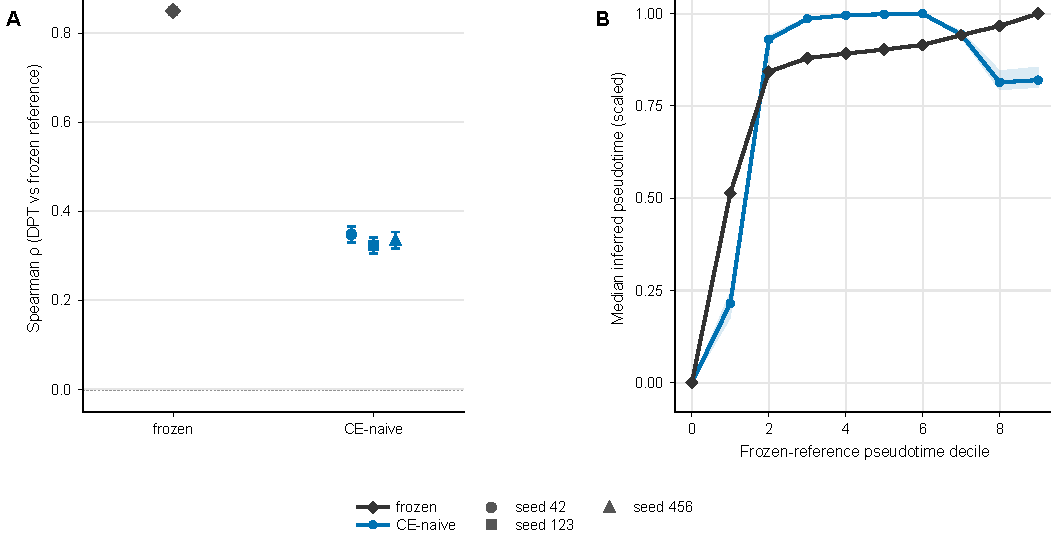
\includegraphics[width=\textwidth]{figureS11_trajectory_continuity}
  \caption{Trajectory inference confirms the geometric dissociation. Diffusion pseudotime on external cells (GSE153515, $n$ = 14,775; three seeds per adapted arm; Methods): left, Spearman $\rho$ between inferred pseudotime and the fixed stage-centroid reference from the frozen representation (individual seeds with bootstrap 95\% CI ranges): frozen representations preserve cell ordering relative to the reference pseudotime ($\rho$ = 0.850, 95\% CI 0.842--0.858) and CE-naive does not ($\rho$ = 0.323--0.348); right, min--max-scaled median inferred pseudotime across frozen-reference pseudotime deciles. For adapted arms, lines show the three-seed mean and shading the per-decile seed range; the frozen reference is a single curve. Seed-marker shapes identify runs in the left panel. Files: \texttt{figures/paper1/figureS11\_trajectory\_continuity.\{pdf,png\}}. Generated by \texttt{scripts/analyze\_trajectory\_continuity.py}.}
  \label{fig:S11}
\end{figure}

% ── Figure S12 ────────────────────────────────────────────────────────────
\begin{figure}[htbp]
  \centering
  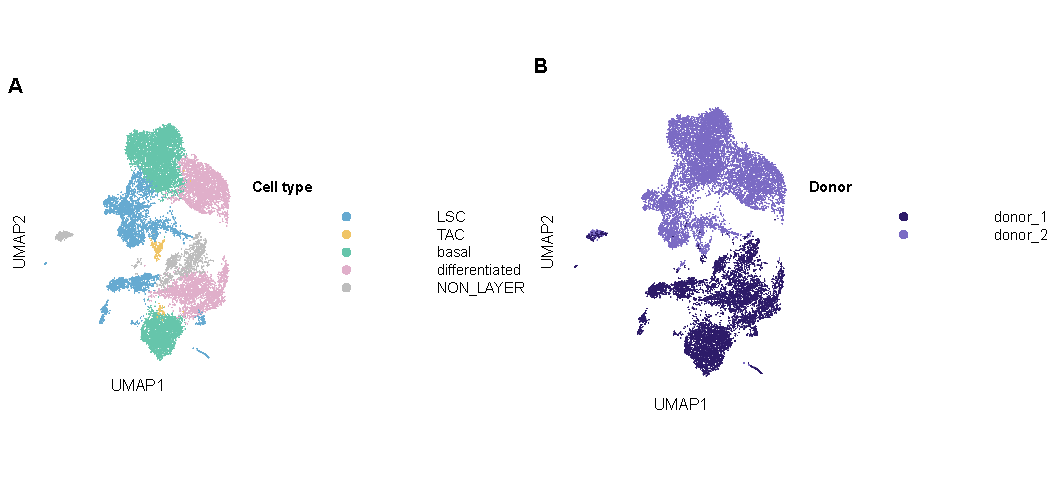
\includegraphics[width=\textwidth]{figureS12_annotation_overview}
  \caption{Annotation of the external test sets. External test annotation (GSE153515; $n$ = 15,827 QC-passing cells from two donors): unsupervised integration and clustering, and DEG-based assignment to four ordered differentiation classes. (A) Cell type and (B) donor on the shared UMAP; the cell-type panel also shows cells assigned \texttt{NON\_LAYER}. Cluster-level annotation detail (marker-set scores and assignment heatmap) is provided as Figure S8. Files: \texttt{figures/paper1/figureS12\_annotation\_overview.\{pdf,png\}}. Generated by \texttt{scripts/figureS12\_annotation\_overview.py}.}
  \label{fig:S12}
\end{figure}

% ── Figure S13 ────────────────────────────────────────────────────────────
\begin{figure}[htbp]
  \centering
  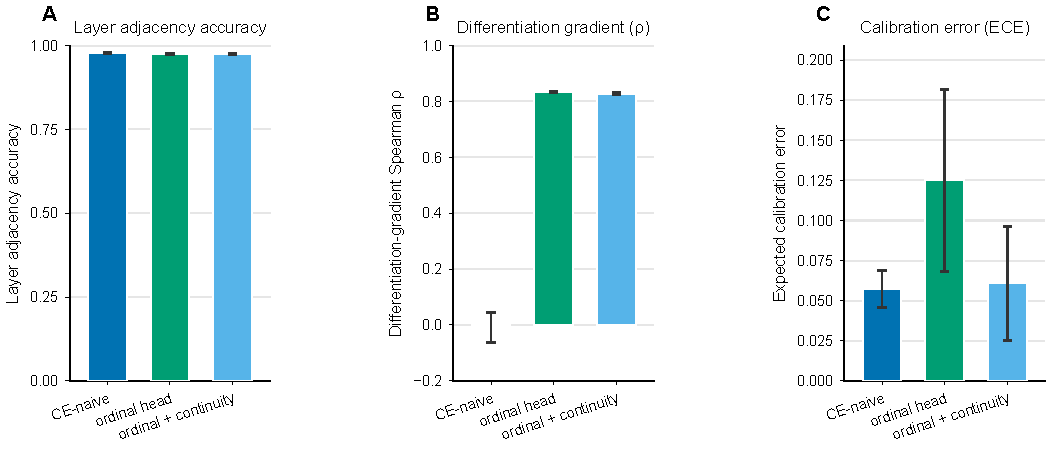
\includegraphics[width=\textwidth]{figureS13_continuity_metrics}
  \caption{Related to Figure 2: Continuity metrics under task adaptation. An ordinal head parameterization preserves the differentiation gradient. (A) Layer adjacency accuracy (LAA). (B) Differentiation-gradient Spearman $\rho$. (C) Expected calibration error (ECE). Bars are three-seed mean $\pm$ SD for CE-naive, ordinal head and ordinal + continuity (n = 14,775 cells per arm). See also Figure S3.}
  \label{fig:S13}
\end{figure}

\clearpage

% ==========================================================================
%  Supplementary Tables
% ==========================================================================
\section*{Supplementary Tables}

% ── Table S1 ──────────────────────────────────────────────────────────────
\needspace{45mm}
\subsection*{Table S1. Related to Table 1: Primary external-test metrics for the naive, HVG/PCA, and frozen-Geneformer arms (per-seed, per-donor, per-class)}
\label{tab:S1}

\textbf{Models.} Three fine-tuned Geneformer-V2-104M checkpoints (naive $\lambda$=0.0, seeds 42/123/456) plus two seed-independent baselines (HVG/PCA logistic probe and frozen Geneformer). Metrics were computed on the external test set (GSE153515, 14,775 epithelial cells). Macro-F1 is donor-level macro F1 with a 95\% bootstrap CI ($n_{\mathrm{boot}}$=1000, seed 42), LAA is layer adjacency accuracy, $\rho$ is the differentiation-gradient rank correlation, and ECE is the expected calibration error over 10 bins.

\textbf{Panel A. Per-seed external-test metrics by training epoch.}

\textbf{Epoch coverage.} Training used \texttt{save\_total\_limit=2}, so the retained checkpoints cover epochs 2--3. Epoch-3 rows reproduce \texttt{results/paper1\_tier\_b\_eval/results\_*.json} exactly for all metrics except ECE, whose binning is noted below.

\medskip
\begingroup
\small
\centering
\resizebox{\textwidth}{!}{%
\begin{tabular}{lcrrlrrrrrrr}
\toprule
Arm & $\lambda$ & Seed & Epoch & Checkpoint & macro-F1 & CI lower & CI upper & LAA & $\rho$ & ECE & Mean train loss\\
\midrule
naive & 0.0 & 42 & 2 & checkpoint-4982 & 0.6564 & 0.6380 & 0.6748 & 0.9762 & $-$0.0483 & 0.0623 & 0.2374\\
naive & 0.0 & 42 & 3 & checkpoint-7473 & 0.6542 & 0.6331 & 0.6753 & 0.9760 & $-$0.0424 & 0.0460 & 0.2143\\
naive & 0.0 & 123 & 2 & checkpoint-4982 & 0.6414 & 0.6115 & 0.6713 & 0.9773 & $-$0.0244 & 0.1188 & 0.2343\\
naive & 0.0 & 123 & 3 & checkpoint-7473 & 0.6420 & 0.6109 & 0.6731 & 0.9777 & $-$0.0360 & 0.0690 & 0.2101\\
naive & 0.0 & 456 & 2 & checkpoint-4982 & 0.6529 & 0.6286 & 0.6773 & 0.9773 & 0.0203 & 0.0900 & 0.2358\\
naive & 0.0 & 456 & 3 & checkpoint-7473 & 0.6515 & 0.6260 & 0.6770 & 0.9767 & 0.0539 & 0.0574 & 0.2127\\
\midrule
hvg\_pca & None & $--$ & $--$ & n/a & 0.6192 & 0.5747 & 0.6637 & 0.9771 & 0.8206 & 0.0145 & $--$\\
frozen\_gf & None & $--$ & $--$ & n/a & 0.4421 & 0.3749 & 0.5093 & 0.9665 & 0.8064 & 0.3010 & $--$\\
\bottomrule
\end{tabular}%
}
\endgroup

\textbf{Notes.}
\begin{itemize}
  \item ECE uses 10 equal-width half-open probability bins \texttt{[lo, hi)} with the final bin closed (\texttt{np.digitize}, \texttt{right=False}, in \texttt{corneal\_fm/evaluation.py} and \texttt{scripts/measure\_percell\_probs.py} \texttt{\_reliability\_bins}). The epoch-3 (final-checkpoint) and HVG/PCA rows follow this convention, and their values are recorded in \texttt{results/paper1\_pipeline\_audit/ece\_corrected.json}.
  \item Epoch-2 rows follow the binning of the locked \texttt{results\_*.json} files.
  \item Scope: this table covers the naive ($\lambda$ = 0), HVG/PCA, and frozen-Geneformer arms, whereas the ordinal arms are reported in Table 1 of the main text and in Table S2.
  \item Mean train loss is aggregated from \texttt{trainer\_state.json} log\_history as per-epoch means over logged steps.
  \item The internal holdout used for the calibration/OOD figures is each run's own prepared holdout export under \texttt{prepared/} (19,922 cells, 6,924 epithelial after removing NON\_LAYER), not the manuscript's donor-disjoint test (20,394 cells / 25 donors).
  \item Generated 2026-08-03 15:01 UTC.
\end{itemize}

\textbf{Panel B. Per-donor macro-F1 on external test (GSE153515).}

\begingroup
\small
\begin{tabular}{lcrr}
\toprule
Arm & Seed & Donor 1 (donor\_1) & Donor 2 (donor\_2)\\
\midrule
HVG/PCA + linear & $--$ & 0.6637 & 0.5747\\
Frozen Geneformer & $--$ & 0.5093 & 0.3749\\
Naive FT ($\lambda$=0) & 42 & 0.6753 & 0.6331\\
 & 123 & 0.6731 & 0.6109\\
 & 456 & 0.6770 & 0.6260\\
 & mean & 0.6751 & 0.6233\\
\bottomrule
\end{tabular}
\endgroup

Note: donor\_1/donor\_2 correspond to GSM4646295/GSM4646296, respectively (assigned from cellranger aggr barcode suffixes $-$1/$-$2 during annotation, per Methods, External test annotation pipeline). External per-donor macro-F1 for HVG/PCA (0.6637/0.5747) and frozen Geneformer (0.5093/0.3749) is from the reference-arm evaluation JSONs (single run, no seeds). With only two donors, the donor-level bootstrap 95\% CI is spanned by the two per-donor values.

\textbf{Panel C. Per-class precision, recall, F1, and support for fine-tuned arms (external test, 3-seed means).}

\begingroup
\small
\begin{tabular}{lccrrrr}
\toprule
Arm & Class & Precision & Recall & F1 & Support & $n_{\mathrm{seeds}}$\\
\midrule
Fine-tune $\lambda$=0 & LSC & 0.9776 & 0.7658 & 0.8588 & 3423 & 3\\
Fine-tune $\lambda$=0 & TAC & 0.0 & 0.0 & 0.0000 & 171 & 3\\
Fine-tune $\lambda$=0 & basal & 0.8041 & 0.9941 & 0.8890 & 6698 & 3\\
Fine-tune $\lambda$=0 & differentiated & 0.9339 & 0.7482 & 0.8306 & 4483 & 3\\
\bottomrule
\end{tabular}
\endgroup

Note: values transcribed verbatim from \texttt{figures/paper1/table\_t4\_per\_class\_metrics.csv} (3-seed means, support = number of cells per class in the external test). Per-class F1 for the reference arms (HVG/PCA, frozen Geneformer) is not tabulated, and per-arm macro-F1 is in Table 1 of the main text. The TAC F1 = 0.0 in all adapted runs reflects class rarity (171/14,775 cells, 1.2\%) with zero true-positive predictions in every seed.

% ── Table S2 ──────────────────────────────────────────────────────────────
\needspace{45mm}
\subsection*{Table S2. Related to Table 1: Label-set and step-budget controls}
\label{tab:S2}

Both arms supervise the same 27{,}878 epithelial training cells with the same four stage labels under the locked donor-disjoint split. They differ in the batched cells and, consequently, in the optimizer-step budget, which is 2{,}616 steps (three epochs over the epithelial subset) in one arm and 7{,}473 steps, matched to the ordinal arm, in the other, so the pair separates the label set from the step budget. Three seeds (42, 123, 456) were run per arm, and evaluation is on the same GSE153515 holdout (14{,}775 cells, two donors).

\medskip
\begingroup
\footnotesize
\setlength{\tabcolsep}{4pt}%
\centering
\begin{tabular}{@{}l c r r r r@{}}
\toprule
Arm & Seed & $\rho$ & Macro-F1 & LAA & ECE\\
\midrule
2{,}616 steps & 42 & 0.2142 & 0.6632 & 0.9794 & 0.0718\\
              & 123 & 0.1413 & 0.6597 & 0.9827 & 0.0774\\
              & 456 & 0.1191 & 0.6583 & 0.9796 & 0.0817\\
              & mean $\pm$ SD & 0.1582 $\pm$ 0.0497 & 0.6604 $\pm$ 0.0025 & 0.9806 $\pm$ 0.0019 & 0.0770 $\pm$ 0.0050\\
\midrule
7{,}473 steps & 42 & 0.2663 & 0.6639 & 0.9779 & 0.0965\\
              & 123 & 0.2293 & 0.6544 & 0.9809 & 0.1091\\
              & 456 & 0.2667 & 0.6545 & 0.9796 & 0.1087\\
              & mean $\pm$ SD & 0.2541 $\pm$ 0.0215 & 0.6576 $\pm$ 0.0054 & 0.9794 $\pm$ 0.0015 & 0.1048 $\pm$ 0.0072\\
\bottomrule
\end{tabular}
\endgroup

\medskip
\noindent\emph{Note:} values transcribed from the per-seed \texttt{eval\_gse153515.json} records under \texttt{results/paper1\_vanzyl/epi4\_ce/} (\texttt{drop\_nonepi} and \texttt{mask\_nonepi}), where $\rho$ is the differentiation-gradient Spearman correlation (Table 1 metric).

% ── Table S3 ──────────────────────────────────────────────────────────────
\needspace{45mm}
\subsection*{Table S3. Related to Figure 2: Layer-resolved differentiation-gradient Spearman $\rho$ (external test, $n$ = 14,775 cells)}
\label{tab:S3}

\begingroup
\small
\centering
\resizebox{\textwidth}{!}{%
\begin{tabular}{lrrrrrrrrrrrrr}
\toprule
Model & L0 & L1 & L2 & L3 & L4 & L5 & L6 & L7 & L8 & L9 & L10 & L11 & L12\\
\midrule
Frozen Geneformer & NaN & 0.4595 & 0.5433 & 0.7656 & 0.7807 & 0.7868 & 0.7642 & 0.6453 & 0.5687 & 0.6221 & 0.6256 & 0.6601 & 0.8064\\
Naive FT ($\lambda$=0), s42 & NaN & 0.4068 & 0.6346 & 0.8380 & 0.8234 & 0.3973 & 0.2052 & 0.1382 & 0.1429 & 0.1938 & 0.1685 & 0.1321 & $-$0.0424\\
Naive FT ($\lambda$=0), s123 & NaN & 0.4093 & 0.5807 & 0.8062 & 0.8042 & 0.5072 & 0.3801 & 0.2659 & 0.3099 & 0.8066 & 0.3665 & 0.1193 & $-$0.0360\\
Naive FT ($\lambda$=0), s456 & NaN & 0.4222 & 0.6570 & 0.8382 & 0.6890 & 0.4633 & 0.3102 & 0.2558 & 0.0582 & 0.3047 & 0.2777 & 0.2579 & $+$0.0539\\
\bottomrule
\end{tabular}%
}
\endgroup

Note: values are the differentiation-gradient Spearman $\rho$ measured at each hidden state (L0 embedding output, L1--L12 Transformer layers), rounded to four decimals from the full-precision data in \texttt{results/paper1\_layerwise\_rho/summary.json} (generated 2026-08-03T04:47:02+00:00). L0 is NaN in all models because the position-0 [CLS] representation of the embedding output is constant across cells, which leaves Spearman $\rho$ undefined. Each model's L12 $\rho$ reproduces the corresponding single-value $\rho$ reported in Table 1 of the main text bit-exactly (absolute difference 0.0, tolerance $1 \times 10^{-6}$, 4/4 passed). Results are reported in Results (Geneformer fine-tuning improves annotation but collapses the differentiation gradient on the same-corpus holdout) and Figure 2, with per-seed curves in Figure S7.

% ── Table S4 ──────────────────────────────────────────────────────────────
\needspace{45mm}
\subsection*{Table S4. Related to Table 1: Frozen-representation probes across single-cell foundation models}
\label{tab:S4}

\begingroup
\footnotesize
\setlength{\tabcolsep}{4pt}%
\centering
\begin{tabular}{@{}>{\raggedright\arraybackslash}p{2.5cm} >{\raggedright\arraybackslash}p{2.4cm} >{\centering\arraybackslash}p{1.8cm} >{\centering\arraybackslash}p{1.8cm} >{\raggedright\arraybackslash}p{2.7cm} >{\raggedright\arraybackslash}p{2.0cm} >{\raggedright\arraybackslash}p{2.6cm}@{}}
\toprule
Model (frozen) & Embedding (dim) & GSE153515 $\rho$ & GSE299152 $\rho$ & GSE153515 probe macro-F1 & GSE299152 probe macro-F1 & Corpus status\\
\midrule
Geneformer-V2-104M & {[}CLS{]} L12 (768) & 0.806 & 0.707 & 0.90 (cell-level); 0.442 (donor-level, Table 1) & 0.114 (donor-level) & GSE153515 in-corpus; GSE299152 post-cutoff out\\
scFoundation (01B-resolution) & official pool\_type=all (3,072) & 0.748 & 0.724 & 0.945 & 0.970 & Unknown (pretraining corpus not publicly enumerated)\\
UCE (33-layer) & CLS hidden state (1,280, L2-norm) & 0.576 & 0.707 & 0.793 & 0.916 & Inferred out-of-corpus (census 2023-04-25)\\
scGPT-human & CLS L12 (512) & 0.219 & 0.172 & 0.851 & 0.893 & out-of-corpus (census 2023-05-15)\\
\bottomrule
\end{tabular}
\endgroup

\textbf{Notes.}
\begin{itemize}
  \item $\rho$ = differentiation-gradient Spearman (layer-centroid PCA axis, LSC $\rightarrow$ TAC $\rightarrow$ basal $\rightarrow$ differentiated), identical to the metric in main-text Table 1, and all $\rho$ values have label-shuffle null $z \ge 94$ ($n$ = 100, seed 42).
  \item Probe macro-F1 = four-class logistic-regression probe (cell-level 80/20 split, five repeats, mean). GSE299152 probe values use present-classes averaging because the TAC class is absent (label counts: LSC 15,921 / TAC 0 / basal 1,099 / differentiated 4,354), since forced four-class averaging would cap scores at 0.75.
  \item Geneformer GSE153515 cell-level probe macro-F1 is 0.90 under the same probe convention as the other models, and its GSE299152 counterpart is the donor-level macro-F1 of 0.114.
  \item UCE values are three-repeat means (seeds 42/123/456) of the stochastic expression-weighted gene sampling. For GSE153515, $\rho$ is 0.5757 (per-repeat 0.5746/0.5746/0.5780) and probe macro-F1 is 0.7932 $\pm$ 0.0076. For GSE299152, $\rho$ is 0.7072 (0.7049/0.7093/0.7075) and probe macro-F1 is 0.9160 $\pm$ 0.0081.
  \item Files: \texttt{results/scgpt\_repro/frozen\_diag/}, \texttt{results/scfoundation\_repro/frozen\_diag/}, \texttt{results/uce\_repro/frozen\_diag/}.
\end{itemize}

% ── Table S5 ──────────────────────────────────────────────────────────────
\needspace{45mm}
\subsection*{Table S5. Related to Methods: Training-atlas composition and provenance record}
\label{tab:S5}

\textbf{Panel A. Constituent studies of the training atlas.}

\begingroup
\small
\begin{tabular}{lr}
\toprule
Study name (Methods, Data sources and preprocessing) & Cell count\\
\midrule
chen\_limbus & 30,699\\
chen\_cornea & 26,158\\
chen\_sclera & 14,205\\
chen\_fetal & 10,046\\
lako\_adult\_GSE155683 & 2,987\\
lako\_fetal\_GSE155683 & 6,985\\
shi\_GSE157474 & 4,099\\
chakravarti\_GSE218123 & 2,493\\
dickman\_GSE186433 & 1,511\\
li\_GSE147979 & 423\\
\bottomrule
\end{tabular}
\endgroup

Note: cell counts verified against the \texttt{obs.study} column of \texttt{data/corneal\_100k\_donor\_split.h5ad} (checked 2026-08-03). The collection aggregates 10 constituent studies spanning corneal, limbal, scleral, and fetal ocular surface tissues, and the lako GSE155683 study contributes two partitions, lako\_adult\_GSE155683 (2,987) and lako\_fetal\_GSE155683 (6,985), which were previously merged as lako\_GSE155683 (9,972). The sum of the 10 listed studies is 99,606, equal to the training partition after the donor-disjoint fair split, and Methods, Data sources and preprocessing lists the same 10 studies. The aggregated atlas totals 120,000 cells with curated cell-type labels (Methods, Data sources and preprocessing), from $\sim$815,000 raw cells before QC, and the training partition holds 99,606 cells from 49 donors while the internal test partition holds 20,394 cells from 25 donors with zero donor overlap.

\textbf{Panel B. Provenance record (transcribed verbatim from \texttt{figures/paper1/table6\_provenance.csv}).}

\begingroup
\small
\centering
\resizebox{\textwidth}{!}{%
\begin{tabular}{lp{3cm}cp{3.5cm}c}
\toprule
Component & Detail & Weights checksum & Corpus & Retrieved\\
\midrule
Model & Geneformer-V2-104M (HuggingFace snapshot 04c2b2e8) & SHA-256 fff5cba2\ldots & Genecorpus-104M ($\sim$104M cells, 2,903 datasets) & 2026-07-23\\
Tokenizer & Geneformer tokenizer (pkl gc104M dicts) & & Genecorpus-104M &\\
Training data & CELLxGENE corpus 0f7d022a (dataset 30127f02) & MD5 39f098\ldots & corneal/limbal scRNA-seq (49 donors, 10 studies) & 2026-07-22\\
External test & GSE153515 (17,587 cells; 15,827 after QC) & & DOIs: 10.1016/\allowbreak j.jtos.2020.12.004, 10.1167/\allowbreak iovs.62.9.36 &\\
\bottomrule
\end{tabular}%
}
\endgroup

Note: the CSV stores truncated checksum prefixes as shown. The full model-weights SHA-256 (\texttt{fff5cba29ddd8792991fa77b4872246fbe548a178cebda3775cdc72b67780e7f}), the full Hugging Face snapshot commit (\texttt{04c2b2e84da7c0f385c3f9ad8f3ec24bab6650e5}) and the full training-atlas MD5 (\texttt{39f098367af95bc3e1ee92528ceb251e}) are the authoritative identifiers for this record.

% ── Table S6 ──────────────────────────────────────────────────────────────
\needspace{45mm}
\subsection*{Table S6. Related to Figure 6: scGPT-human same-corpus arms --- per-seed test-donor metrics across budgets}
\label{tab:S6}

Test-donor metrics were measured on the locked van Zyl same-corpus test donor Hu0216 (n = 20,158 epithelial cells, three-tier LSC $\rightarrow$ basal $\rightarrow$ differentiated axis, per Methods). Here $\rho$ (L2) is the differentiation-gradient Spearman correlation on L2-normed embeddings, macro-F1 is the test-donor macro-F1 from single-test-donor cell-level statistics, and the mean $\pm$ SD entries are the arithmetic mean and sample SD across the listed seeds.

\medskip
\begingroup
\small
\centering
\resizebox{\textwidth}{!}{%
\begin{tabular}{llrr}
\toprule
Arm / checkpoint & Seed & $\rho$ (L2) & Macro-F1 \\
\midrule
CE, 3 epochs, final & 42 & 0.2727 & 0.9325 \\
CE, 3 epochs, final & 123 & 0.7570 & 0.9207 \\
CE, 3 epochs, final & 456 & 0.6364 & 0.9144 \\
CE, 3 epochs, final & mean $\pm$ SD & 0.5554 $\pm$ 0.2521 & 0.9225 $\pm$ 0.0092 \\
\addlinespace[4pt]
Ordinal head, 3 epochs, final & 42 & 0.6471 & 0.9594 \\
Ordinal head, 3 epochs, final & 123 & 0.9071 & 0.9504 \\
Ordinal head, 3 epochs, final & 456 & 0.9021 & 0.9663 \\
Ordinal head, 3 epochs, final & mean $\pm$ SD & 0.8188 $\pm$ 0.1487 & 0.9587 $\pm$ 0.0080 \\
\addlinespace[4pt]
CE, 15 epochs, best-val & 42 & 0.3373 & 0.9313 \\
CE, 15 epochs, best-val & 123 & 0.5774 & 0.9419 \\
CE, 15 epochs, best-val & 456 & 0.4039 & 0.9201 \\
CE, 15 epochs, best-val & mean $\pm$ SD & 0.4395 $\pm$ 0.1240 & 0.9311 $\pm$ 0.0109 \\
\addlinespace[4pt]
CE, 15 epochs, final & 42 & $-0.0908$ & 0.9038 \\
CE, 15 epochs, final & 123 & 0.8329 & 0.8826 \\
CE, 15 epochs, final & 456 & 0.7647 & 0.8773 \\
CE, 15 epochs, final & 789 & 0.3671 & 0.9433 \\
CE, 15 epochs, final & 2024 & 0.7474 & 0.8887 \\
CE, 15 epochs, final & mean $\pm$ SD & 0.5243 $\pm$ 0.3892 & 0.8991 $\pm$ 0.0266 \\
\addlinespace[4pt]
LoRA, 15 epochs, best-val & 42 & 0.8380 & 0.9319 \\
LoRA, 15 epochs, best-val & 123 & 0.8755 & 0.9392 \\
LoRA, 15 epochs, best-val & 456 & 0.8861 & 0.9314 \\
LoRA, 15 epochs, best-val & mean $\pm$ SD & 0.8665 $\pm$ 0.0253 & 0.9342 $\pm$ 0.0044 \\
\addlinespace[4pt]
LoRA, 15 epochs, final & 42 & 0.8265 & 0.9523 \\
LoRA, 15 epochs, final & 123 & 0.8407 & 0.9352 \\
LoRA, 15 epochs, final & 456 & 0.8638 & 0.9430 \\
LoRA, 15 epochs, final & mean $\pm$ SD & 0.8436 $\pm$ 0.0188 & 0.9435 $\pm$ 0.0086 \\
\addlinespace[4pt]
Ordinal head + LoRA, 15 epochs, best-val & 42 & 0.9247 & 0.9662 \\
Ordinal head + LoRA, 15 epochs, best-val & 123 & 0.9242 & 0.9681 \\
Ordinal head + LoRA, 15 epochs, best-val & 456 & 0.9235 & 0.9633 \\
Ordinal head + LoRA, 15 epochs, best-val & mean $\pm$ SD & 0.9241 $\pm$ 0.0006 & 0.9659 $\pm$ 0.0024 \\
\addlinespace[4pt]
Ordinal head + LoRA, 15 epochs, final & 42 & 0.9247 & 0.9662 \\
Ordinal head + LoRA, 15 epochs, final & 123 & 0.9209 & 0.9583 \\
Ordinal head + LoRA, 15 epochs, final & 456 & 0.9223 & 0.9659 \\
Ordinal head + LoRA, 15 epochs, final & mean $\pm$ SD & 0.9226 $\pm$ 0.0019 & 0.9635 $\pm$ 0.0045 \\
\bottomrule
\end{tabular}%
}
\endgroup

\textbf{Notes.}
\begin{itemize}
  \item CE rows are naive cross-entropy fine-tuning, and ordinal-head rows use the unconditional cumulative-threshold ordinal head. The 3-epoch CE and ordinal-head arms are final-epoch checkpoints. The 15-epoch arms (CE, LoRA, ordinal head + LoRA) follow the official scGPT 15-epoch protocol with best-validation checkpoint selection, and their final-epoch checkpoints are shown for sensitivity, while the CE15-final block includes the two additional seeds 789 and 2024. The full convergence checkpoints are tabulated in Table S7.
  \item Per-seed values were compiled from the locked scGPT-human van Zyl run summaries in the released artifact bundle (\texttt{results/paper1\_vanzyl/run6/eval/summary\_vanzyl\_6run.json}, \texttt{results/paper1\_vanzyl/baselines/baselines\_rho.json} and \texttt{results/paper1\_vanzyl/corn\_lora/summary.json}), while the LoRA15-final and ordinal-head + LoRA final per-seed values were read from the checkpoint \texttt{args.json} files under \texttt{artifacts/paper1\_vanzyl/run6/lora\_v2/checkpoints/} and \texttt{artifacts/paper1\_vanzyl/corn\_lora/checkpoints/} (\texttt{test\_donor\_eval.final\_epoch}).
\end{itemize}

% ── Table S7 ──────────────────────────────────────────────────────────────
\needspace{45mm}
\subsection*{Table S7. Related to Figure 6: scGPT-human convergence checkpoints (van Zyl, test donor Hu0216)}
\label{tab:S7}

\begingroup
\small
\centering
\resizebox{\textwidth}{!}{%
\begin{tabular}{lrrrrrr}
\toprule
Checkpoint & Seed & Macro-F1 & 95\% CI & $\rho$ & $z$ & Val $\rho$ peak (epoch) \\
\midrule
Best-val & 42 & 0.9313 & [0.9272, 0.9351] & 0.3373 & 36.4 & 0.730 (3) \\
Best-val & 123 & 0.9419 & [0.9384, 0.9454] & 0.5774 & 66.3 & 0.852 (3) \\
Best-val & 456 & 0.9201 & [0.9158, 0.9243] & 0.4039 & 41.8 & 0.778 (6) \\
Best-val mean & & 0.9311 & [0.9041, 0.9581] ($t$-interval, 3 seeds) & 0.4395 & 48.2 & \\
\addlinespace[4pt]
Final-epoch & 42 & 0.9038 & [0.8992, 0.9083] & $-0.0908$ & $-12.2$ & \\
Final-epoch & 123 & 0.8826 & [0.8774, 0.8876] & 0.8329 & 90.2 & \\
Final-epoch & 456 & 0.8773 & [0.8722, 0.8826] & 0.7647 & 85.1 & \\
Final-epoch & 789 & 0.9433 & [0.9399, 0.9467] & 0.3671 & 39.0 & \\
Final-epoch & 2024 & 0.8887 & [0.8836, 0.8932] & 0.7474 & 82.7 & \\
Final-epoch mean & & 0.8991 & observed range: $-0.091$ to $0.833$ & 0.5243 & 57.0 & \\
\bottomrule
\end{tabular}%
}
\endgroup

Note: scGPT-human same-corpus arm (van Zyl, pre-registered test donor Hu0216, n = 20,158 epithelial cells). Convergence-arm checkpoints were evaluated per seed on the test donor, using macro-F1 with a cell-level bootstrap 95\% CI (n = 1,000, seed 42), differentiation-gradient $\rho$ on L2-normed embeddings, and label-shuffle $z$ with n = 100. The validation-$\rho$ peak and its epoch come from the per-epoch trajectories, with the best-validation epoch chosen by validation macro-F1. The frozen baseline on the test donor is $\rho$ = 0.789 with $z$ = 99.3, and because a single test donor makes donor-level statistics degenerate, cell-level bootstrap is used throughout (Methods). The final-epoch mean entry is the observed five-seed range rather than a confidence interval, because per-seed outcomes span collapse to retention. The Best-val mean entry is a 95\% $t$-interval across the three seed means ($n$ = 3, $t_{2,0.975}$ = 4.303), distinct from the cell-level bootstrap CIs on the per-seed rows. Mean $z$ values are arithmetic means of the per-seed $z$ values (three seeds for Best-val, five for Final-epoch).

% ── Table S8 ──────────────────────────────────────────────────────────────
\needspace{45mm}
\subsection*{Table S8. Related to Figure 6: Geneformer official-budget control}
\label{tab:S8}

\begingroup
\small
\centering
\resizebox{\textwidth}{!}{%
\begin{tabular}{lrrr}
\toprule
Budget & $\rho$ per seed & $\rho$ mean & Macro-F1 per seed \\
\midrule
Official one epoch (42/123/456) & 0.201 / 0.144 / $-0.057$ & 0.096 & 0.6397 / 0.6414 / 0.6357 \\
Official one epoch (789/2024/31415) & 0.102 / 0.091 / $-0.133$ & 0.020 & 0.6554 / 0.6387 / 0.6522 \\
Official one epoch (all six seeds) & --- & 0.058 & --- \\
Main protocol (three epochs) & $-0.042$ / $-0.036$ / $+0.054$ & $-0.008$ & 0.6542 / 0.6420 / 0.6515 \\
\bottomrule
\end{tabular}%
}
\endgroup

Note: Geneformer official-budget control (same-corpus GSE153515, n = 14,775 epithelial cells). Naive cross-entropy fine-tuning at the official one-epoch budget (all six pre-registered seeds: 42, 123, 456, plus the E3 seeds 789, 2024, 31415) is compared with the main three-epoch protocol, reporting per-seed differentiation-gradient $\rho$ (raw) with per-budget seed means and donor-level macro-F1 per seed. The three-epoch reference is the pre-registered main-protocol arm (Table 1 of the main text).

% ── Table S9 ──────────────────────────────────────────────────────────────
\needspace{45mm}
\subsection*{Table S9. Related to Figure 6: CellPLM arms}
\label{tab:S9}

\textbf{Panel A. van Zyl same-corpus arm (test donor Hu0216; n = 20,158 epithelial cells).}

\medskip
\begingroup
\small
\centering
\resizebox{\textwidth}{!}{%
\begin{tabular}{lrrr}
\toprule
Arm & Seed & $\rho$ (L2) & Macro-F1 \\
\midrule
Naive CE (mean $\pm$ sample SD) & 42/123/456 & $-0.007096 \pm 0.034595$ & $0.972806 \pm 0.000294$ \\
\addlinespace[4pt]
Ordinal head & 42 & 0.920300 & 0.973734 \\
Ordinal head & 123 & 0.916323 & 0.971312 \\
Ordinal head & 456 & 0.917447 & 0.973352 \\
Ordinal head (mean $\pm$ sample SD) & 42/123/456 & $0.918023 \pm 0.002050$ & $0.972799 \pm 0.001302$ \\
\bottomrule
\end{tabular}%
}
\endgroup

\textbf{Panel B. Two-seed consistency replication.}

\medskip
\begingroup
\small
\centering
\begin{tabular}{llrr}
\toprule
Test setting & Arm & $\rho$ (L2) & Macro-F1 \\
\midrule
Epidermis (cross-tissue) & Naive, 2-seed mean $\pm$ SD & $0.835 \pm 0.006$ & $0.782 \pm 0.007$ \\
Epidermis (cross-tissue) & Frozen axis & 0.094 & --- \\
Leave-one-donor Hu0220 & Naive, 2-seed mean $\pm$ SD & $0.659 \pm 0.008$ & $0.923 \pm 0.005$ \\
Leave-one-donor Hu0220 & Frozen axis & 0.814 & --- \\
\bottomrule
\end{tabular}
\endgroup

\textbf{Panel C. Parameter-efficient and layerwise analyses (single seed).} LoRA adaptation of CellPLM (QKV projections, r = 8, $\alpha$ = 16) achieved $\rho$ = 0.873 (label-shuffle $z$ = 132.4) with macro-F1 = 0.958 on the van Zyl test donor. Layerwise analysis localized the naive collapse to the entry layer: naive L1 $\rho$ dropped from 0.906 at the embedder output to 0.118, whereas frozen L1 remained 0.771.

\textbf{Notes.}
\begin{itemize}
  \item Panel A: the naive CE reference and the ordinal-head values are from \texttt{summary\_vanzyl\_cellplm\_corn.json} (archived, released artifact bundle), and the naive CE mean $\pm$ SD is reproduced by the locked per-seed $\rho$ values in \texttt{results/paper1\_vanzyl/sensitivity/sensitivity\_summary.json} (\texttt{locked\_metric\_rho}). The frozen CellPLM baseline on the same test donor is reported in the main text.
  \item Panel B: two-seed (42 and 123) consistency values come from \texttt{results/paper1\_vanzyl/cellplm\_consistency/summary\_all.json} (epidermis and loo220 blocks), and the frozen-axis values are single-run references from the same file.
  \item Panel C: the LoRA value comes from \texttt{results/paper1\_vanzyl/\allowbreak cellplm\_lora/seed42/seed42.json} (eval block), and the layerwise L0/L1 values come from \texttt{results/paper1\_vanzyl/\allowbreak cellplm\_layerwise/cellplm\_layerwise\_rho.json} (per-config frozen/naive).
\end{itemize}

% ── Table S10 ─────────────────────────────────────────────────────────────
\needspace{45mm}
\subsection*{Table S10. Related to Table S12: Classical baselines}
\label{tab:S10}

Strong classical baselines on the locked van Zyl test donor (Hu0216, n = 20,158 epithelial cells, three-tier axis, PREREG \S8 split). Here $\rho_{\text{normed}}$ is the differentiation-gradient Spearman correlation on L2-normed embeddings, probe\_f1 is the split self-probe macro-F1 over five repeats, and transfer\_f1 is the train-fit probe macro-F1.

\medskip
\begingroup
\small
\centering
\resizebox{\textwidth}{!}{%
\begin{tabular}{lrrrl}
\toprule
Arm & $\rho_{\text{normed}}$ & probe\_f1 & transfer\_f1 & Gate conclusion \\
\midrule
harmony\_nh2000\_npc50 & 0.8401 & 0.9529 & 0.9363 & Q1 pass; Q2 pass \\
hvg\_pca\_nh2000\_npc100 & 0.8495 & 0.9526 & 0.9400 & Q1 pass; Q2 pass \\
hvg\_pca\_nh2000\_npc50 & 0.8416 & 0.9534 & 0.9385 & Q1 pass; Q2 pass \\
hvg\_pca\_nh5000\_npc100 & 0.8522 & 0.9664 & 0.9577 & Q1 pass; Q2 pass \\
hvg\_pca\_nh5000\_npc50 & 0.8491 & 0.9660 & 0.9580 & Q1 pass; Q2 pass \\
scvi\_nlatent128 & 0.8645 & 0.9729 & 0.9451 & Q1 pass; Q2 pass \\
\midrule
Overall & --- & --- & --- & Q1 all true; Q2 all within 0.10; Q3 = false (highest baseline $\rho$ 0.8645) \\
\bottomrule
\end{tabular}%
}
\endgroup

\textbf{Notes.}
\begin{itemize}
  \item Source: \texttt{results/paper1\_vanzyl/baselines/baselines\_rho.json} (\texttt{comparison\_table} and \texttt{gates} blocks). The gate rules are Q1, $\rho_{\text{baseline}} \ge 0.5$ (all six true), Q2, $\rho_{\text{baseline}}$ within 0.10 of the frozen scFM gradient (all six true), and Q3, the frozen scFM gradient exceeds every baseline (false, because the highest baseline $\rho_{\text{normed}}$ is 0.8645 for scvi\_nlatent128).
  \item Harmony limitation (transcribed from the source): the test donor participates in the batch-correction fit, which is standard integration usage, whereas the frozen scFM sees no test donor, so any baseline advantage is conservative for scFM.
\end{itemize}

\newpage

% ── Table S11 ─────────────────────────────────────────────────────────────
\needspace{45mm}
\subsection*{Table S11. Related to Figure 6: CellPLM training-budget dose response}
\label{tab:S11}

\medskip
\begingroup
\small
\centering
\resizebox{\textwidth}{!}{%
\begin{tabular}{llrrrr}
\toprule
Arm & Epochs per seed & $\rho$: 42 / 123 / 456 & $\rho$ mean $\pm$ SD & Macro-F1: 42 / 123 / 456 & Macro-F1 mean $\pm$ SD \\
\midrule
Frozen (unfitted) & --- & --- & 0.8652 & --- & --- \\
\addlinespace[4pt]
Naive CE & 3 / 3 / 3 & 0.8804 / 0.8665 / 0.8908 & $0.8792 \pm 0.0122$ & 0.8635 / 0.7823 / 0.8583 & $0.8347 \pm 0.0454$ \\
Naive CE & 15 / 15 / 15 & 0.8127 / 0.8969 / 0.8770 & $0.8622 \pm 0.0440$ & 0.9593 / 0.9652 / 0.9531 & $0.9592 \pm 0.0060$ \\
Naive CE & 30 / 30 / 30 & 0.6701 / 0.8257 / 0.8413 & $0.7791 \pm 0.0946$ & 0.9719 / 0.9697 / 0.9721 & $0.9712 \pm 0.0014$ \\
Naive CE & 60 / 60 / 60 & 0.4573 / $-0.0285$ / $-0.0617$ & $0.1223 \pm 0.2905$ & 0.9730 / 0.9707 / 0.9725 & $0.9721 \pm 0.0012$ \\
Naive CE & 83 / 118 / 97 & $-0.0464$ / 0.0187 / 0.0064 & $-0.0071 \pm 0.0346$ & 0.9725 / 0.9730 / 0.9730 & $0.9728 \pm 0.0003$ \\
\addlinespace[4pt]
Ordinal + LoRA & 15 / 15 / 15 & 0.9190 / 0.9246 / 0.9241 & $0.9226 \pm 0.0031$ & 0.9023 / 0.9307 / 0.9101 & $0.9144 \pm 0.0147$ \\
Ordinal + LoRA & 154 / 143 / 454 & 0.9216 / 0.9220 / 0.9215 & $0.9217 \pm 0.0003$ & 0.9518 / 0.9468 / 0.9511 & $0.9499 \pm 0.0027$ \\
\addlinespace[4pt]
Ordinal head & 78 / 123 / 129 & 0.9203 / 0.9163 / 0.9174 & $0.9180 \pm 0.0021$ & 0.9737 / 0.9713 / 0.9734 & $0.9728 \pm 0.0013$ \\
\bottomrule
\end{tabular}%
}
\endgroup

\textbf{Notes.}
\begin{itemize}
  \item CellPLM v1.0.0 fine-tuning on the van Zyl same-corpus arm, with the pre-registered test donor Hu0216 (n = 20,158 epithelial cells) and seeds in the order 42 / 123 / 456. Here $\rho$ is the differentiation-gradient Spearman correlation on L2-normalised latents, and macro-F1 is donor-level on the test donor. SD is the sample SD across the three seeds (ddof = 1). The frozen reference is the unfitted pretrained model evaluated once on the same test cells (single run, no interval), which yields a test-donor $\rho$ rather than a validation $\rho$.
  \item Rows with three equal epoch counts ran a fixed budget. The two ``convergence'' rows used the official pipeline defaults (2,000-epoch cap, early stopping at es = 200, patience 25) and stopped at different epochs per seed, so the count differs by seed and is listed in the order 42 / 123 / 456. One ordinal + LoRA seed continued to 454 epochs without early stopping.
  \item The 3-, 15-, 30- and 60-epoch rows and both ordinal + LoRA rows were added on 2026-10-19, while the 83 / 118 / 97 naive-CE and 78 / 123 / 129 ordinal-head rows are the pre-registered main-protocol runs. Sources are \texttt{results/paper1\_vanzyl/cellplm\_e\{3,15,30,60\}/seed*/seed*.json}, \texttt{results/paper1\_vanzyl/cellplm/seed*/seed*.json}, \texttt{results/paper1\_vanzyl/cellplm/corn/seed*/seed*.json}, \texttt{results/paper1\_vanzyl/cellplm\_corn\_lora/seed*/seed*.json} and \texttt{results/paper1\_vanzyl/cellplm\_corn\_lora\_conv/seed*/seed*.json}. Training used \texttt{run\_cellplm\_vanzyl\_e3.py} and \texttt{run\_cellplm\_corn\_lora.py}, with analysis identical to Table S9.
\end{itemize}

\newpage

% ── Table S12 ─────────────────────────────────────────────────────────────
\needspace{45mm}
\subsection*{Table S12. Related to Figure 6: Geometry-preserving recipes on the scGPT-human van Zyl same-corpus test donor (n = 20{,}158 epithelial cells), grouped by epoch budget and checkpoint convention}
\label{tab:S12}

\begingroup
\small
\centering
\begin{tabular}{llcc}
\toprule
Budget / checkpoint & Arm & $\rho$ (L2) & Macro-F1 \\
\midrule
\multicolumn{2}{l}{Frozen (single run)} & 0.789 & 0.969\textsuperscript{\ddag} \\
\addlinespace[4pt]
3 epochs / final & CE-naive & 0.555 (0.252) & 0.923 (0.009) \\
3 epochs / final & Ordinal head & 0.819 (0.149) & 0.959 (0.008) \\
\addlinespace[4pt]
15 epochs / best-val & CE-naive & 0.440 (0.124) & 0.931 (0.011) \\
15 epochs / best-val & LoRA-only & 0.867 (0.025) & 0.934 (0.004) \\
15 epochs / best-val & Ordinal + LoRA & 0.924 (0.001) & 0.966 (0.002) \\
\bottomrule
\end{tabular}
\endgroup

\medskip
\noindent\emph{Note:} Values are three-seed means (seeds 42/123/456) with sample SD in parentheses for test-donor differentiation-gradient $\rho$ on L2-normed embeddings and for macro-F1, while frozen is a single run. $\ddag$Frozen macro-F1 uses a within-test-donor self-probe, whereas adapted macro-F1 measures donor transfer.

\newpage

% ==========================================================================
%  Data S1–S3
% ==========================================================================
\section*{Data S1--S3 and Code Availability}
\label{sec:data}

\textbf{Data S1. Layer-resolved differentiation-gradient $\rho$ (raw values).} \texttt{results/paper1\_layerwise\_rho/summary.json} plus the per-model files \texttt{layerwise\_rho\_*.json} (13 hidden states each, full precision, with the directory README listing every file including the archived runs not reported in this paper). Measured by \texttt{scripts/measure\_layerwise\_rho.py}.

\textbf{Data S2. Per-cell predictions and embeddings.} Per-cell arrays containing ground-truth labels, predicted labels, 4-class probabilities, and CLS embeddings for all 7 Geneformer-based models on both the external test set and the internal holdout. See \texttt{results/paper1\_tier\_b\_eval/}, where the README lists the \texttt{percell\_*.npz} files, each with a \texttt{.meta.json} sidecar, and the directory also retains the archived runs not reported in this paper. The compressed arrays are $\sim$31--60 MB each and are available on request rather than distributed with the repository. Every archived per-cell sanity gate (macro-F1/CI/LAA/$\rho$/ECE) passed bit-exact against \texttt{results\_*.json} (tolerance $1 \times 10^{-6}$). Generated by \texttt{scripts/measure\_percell\_probs.py}. Evaluation JSONs alongside: \texttt{results/paper1\_tier\_b\_eval/results\_\{0.0,0.5\}\_\{42,123,456\}.json}, \texttt{results\_epoch2\_\{0.0,0.5\}\_\{42,123,456\}.json}, \texttt{results\_frozen\_gf.json}, \texttt{results\_hvg\_pca.json}, \texttt{summary.csv}.

\textbf{Data S3. Fair-split manifest.} \texttt{results/paper1\_fair\_split/manifest.json}: deterministic donor-disjoint split (seed = 42), 99,606 train cells / 49 donors, 20,394 test cells / 25 donors, zero donor overlap, SHA-256 checksums of the train/test h5ad files (generated 2026-07-31).

\textbf{Code availability.} The evaluation pipeline is \texttt{scripts/run\_tier\_b\_eval.py} and \texttt{scripts/run\_tier\_b\_baselines.py}, with per-cell extraction and calibration/OOD in \texttt{scripts/measure\_percell\_probs.py}, layer-resolved $\rho$ in \texttt{scripts/measure\_layerwise\_rho.py}, and external-test annotation in \texttt{scripts/protocol\_15\_annotate\_gse153515.py}. Metric implementations: \texttt{corneal\_fm/evaluation.py} (donor-level macro-F1 with bootstrap CI, LAA, differentiation-gradient Spearman $\rho$, ECE). The evaluation protocol configuration was locked before evaluation: \texttt{config/external\_test\_gse153515.yml} (locked 2026-07-31). Random seeds: 42, 123, 456. Figure CSV sources: \texttt{figures/paper1/} (\texttt{table\_t3\_primary\_endpoint.csv}, \texttt{table\_t4\_per\_class\_metrics.csv}, \texttt{table\_t5\_secondary\_endpoints.csv}, \texttt{table\_t7\_seed\_reproducibility.csv}, \texttt{table6\_provenance.csv}, \texttt{figure*\_*.csv}).

% ==========================================================================
%  Supplementary Methods
% ==========================================================================
\newpage
\section*{Supplementary Methods: configuration, provenance and software details}
\label{sec:suppmethods}

This block records the configuration, model snapshots, weight hashes, recorded digests, software environment and audit parameters that the main-text Methods refers to. Every value is reproduced verbatim from the main-text source; relocation does not alter it.

\subsection*{SM1. Training-atlas file identifier and version lock}
The training atlas was downloaded as file \texttt{30127f02-d0b9-4b56-bf4c-e5b77e4989bd.h5ad} (10.29 GB; the recorded MD5 is tabulated in Table S5 and in Data and Code Availability), which identifies the dataset version used here. That version follows schema 7.1.0 and was published on 2025-05-05. The data download (2026-07-22), the model retrieval (2026-07-23), the model and AnnData checksums, and the fair-split manifest were version-locked before adaptation.

\subsection*{SM2. External-test annotation configuration}
GSE153515 labels used parameters locked in \texttt{config/external\_test\_gse153515.yml}, and donor identities were recovered from the 10x barcode suffix convention. Highly variable gene selection, log-normalization, scaling, and PCA were followed by Harmony correction with 30 PCs and Leiden clustering at resolution 0.6, producing 16 clusters, and cluster-specific differentially expressed genes were identified by the Wilcoxon rank-sum test.

GSE299152 used the corresponding pipeline with \texttt{config/external\_test\_gse299152.yml}, in which endothelial and stromal marker sets were added to the \texttt{NON\_LAYER} gate and Leiden clustering ran at resolution 0.7, yielding 15 clusters. Programmatic checks against the CELLxGENE Discover API found no shared GEO accession, donor identifier, or dataset hash between either external test and the ten adaptation-atlas studies.

\subsection*{SM3. Model snapshots, weight hashes and inference settings}
Table SM1 collects the checkpoint, snapshot and hash identifiers and the inference settings for the five model families. The Geneformer snapshot and weight digest are tabulated in Table S5, and the public accessions are restated in Data and Code Availability.

\paragraph*{Table SM1. Model and checkpoint registry.}
\begingroup
\small
\centering
\resizebox{\textwidth}{!}{%
\begin{tabular}{@{}>{\raggedright\arraybackslash}p{2.8cm}>{\raggedright\arraybackslash}p{5.0cm}>{\raggedright\arraybackslash}p{1.8cm}>{\raggedright\arraybackslash}p{8.4cm}@{}}
\toprule
Model & Checkpoint / snapshot & Hash prefix & Inference settings\\
\midrule
Geneformer-V2-104M & Hugging Face model hub (\texttt{ctheodoris/Geneformer}); snapshot and weights in Table S5 & Table S5 & BertForMaskedLM encoder with 12 layers, 12 attention heads, hidden dimension 768 and vocabulary size 20,275; \texttt{[CLS]} L12 embedding (768 dimensions).\\
scGPT-human & \texttt{perturblab/scgpt-human}, scgpt 0.2.5, git commit \texttt{cebd6fae} & git commit & 60,697-gene vocabulary, \texttt{append\_cls=True}, maximum sequence length 1,200 with CLS first; \texttt{[CLS]} L12 embedding (512 dimensions).\\
scFoundation & 01B-resolution checkpoint, \texttt{genbio-ai/scFoundation} mirror & \texttt{9f40bf32} & Entry point \texttt{get\_embedding.py} with \texttt{input\_type=singlecell}, \texttt{output\_type=cell}, \texttt{pool\_type=all}, \texttt{tgthighres=a5}, \texttt{pre\_normalized=F}, \texttt{version=ce}; 3,072-dimensional cell embedding.\\
UCE & 33-layer checkpoint \texttt{33l\_8ep\_1024t\_1280.torch}, Figshare DOI \texttt{10.6084/\allowbreak m9.figshare.24320806} & \texttt{3f458726} & \texttt{eval\_single\_anndata.py} under human species; expression-weighted sampling of 1,024 genes per cell with replacement; padding length 1,536; 1,280-dimensional CLS embedding after L2 normalization.\\
CellPLM & v1.0.0 & --- & Latent VAE mean (LAT); training and adaptation settings in Table SM2.\\
\bottomrule
\end{tabular}%
}
\endgroup

The four-class logistic-regression probes used a cell-level 80/20 split repeated five times and reported mean macro-F1. On GSE153515, HGNC mapping resolved 10,379 of 10,605 ENSEMBL identifiers. Among the 9,175 vocabulary-matched genes, 32 (0.35\%) carried post-download HGNC renamings, none a core corneal marker, and these renamings did not alter the model input. scFoundation raw counts were aligned to the 19,264-gene HGNC vocabulary, matching 9,162 of 9,175 input genes for GSE153515 and 10,296 of 11,274 for GSE299152, and unmatched vocabulary entries were zero-filled.

\subsection*{SM4. Training hyperparameters by arm}
Table SM2 collects the per-arm training configuration. The Geneformer arms share one optimizer setting, the scGPT-human arms share another, and the CellPLM arms use a third with an adapted-LoRA variant.

\paragraph*{Table SM2. Training and adaptation hyperparameters by arm.}
\begingroup
\footnotesize
\setlength{\tabcolsep}{3pt}%
\centering
\begin{tabular}{@{}>{\raggedright\arraybackslash}p{2.7cm}>{\raggedright\arraybackslash}p{1.7cm}>{\raggedright\arraybackslash}p{1.4cm}>{\raggedright\arraybackslash}p{2.0cm}>{\raggedright\arraybackslash}p{1.55cm}>{\raggedright\arraybackslash}p{1.85cm}>{\raggedright\arraybackslash}p{5.1cm}@{}}
\toprule
Arm & Learning rate & Weight decay & Batch (device $\times$ accum) & Precision & Schedule & Budget / other\\
\midrule
Geneformer (adapted arms 1--7) & $5\times10^{-5}$ & 0.001 & 8 $\times$ 4 (effective 32) & bfloat16 & 500 linear warmup & 3 epochs; 7{,}473 steps, or 2{,}616 for the epithelial-only label-set control; gradient checkpointing\\
scGPT-human CE & $5\times10^{-5}$ & 0.001 & 8 $\times$ 4 & bfloat16 & 500 linear warmup & 3 or 15 epochs; maximum sequence length 4{,}253; 30 author-assigned labels\\
scGPT ordinal + LoRA & $5\times10^{-5}$ & 0.001 & 8 $\times$ 4 & bfloat16 & 500 linear warmup & 15 epochs; 0.528M-parameter head and 0.295M adapter parameters\\
CellPLM & $5\times10^{-3}$ ($5\times10^{-4}$ embedder) & $10^{-7}$ & --- & --- & plateau scheduling & 2{,}000-epoch cap, \texttt{es=200}, \texttt{patience=25}; HVG 3{,}000 $\rightarrow$ 2{,}399 panel genes\\
CellPLM LoRA & --- & --- & --- & --- & --- & \texttt{Flow\_Attention} projections, $r=8$, $\alpha=16$\\
\bottomrule
\end{tabular}
\endgroup

Checkpoints were selected by validation F1 and saved as \texttt{model\_best\_valid.pt}. Displayed seed-42 checkpoints and their frozen references represent individual runs, and geometry used the shared stage-rank endpoint. Recipe summaries used the three-seed mean and sample SD ($\mathrm{ddof}=1$). Each longer-budget scGPT cross-entropy epoch saved a checkpoint and recorded validation macro-F1, raw and L2-normalized gradient correlations, and a 100-replicate label-shuffle $z$-score, and selection used the checkpoint with the highest validation macro-F1 while the final checkpoint was retained separately. Layer-resolved measurements covered the embedder output (L0), four Flowformer layers (L1--L4) and the latent VAE mean (LAT).

The revised training reference axis used \texttt{corneal\_fm/axis\_ref.py} in mode \texttt{centroid\_pca}, and the original marker-score mode was retained for reference. Arms 6 and 7 ran with the locked fair-split manifest and the strict-fair checks used by the other adapted arms, with evaluation on the same GSE153515 holdout and the same metrics. The internal split, the external source-separated tests and the van Zyl donor split were distinct evaluation designs.

The preregistered frozen-axis gate G1 required $\rho\ge0.5$ and label-shuffle $z\ge3$, and the revised training-adequacy gate G0 required $\mathrm{F1}_{\mathrm{ce}}\ge0.55$ together with $\mathrm{F1}_{\mathrm{ce}}\ge\mathrm{F1}_{\mathrm{frz}}-0.10$ at the historical $\mathrm{F1}_{\mathrm{frz}}=0.9494$. That historical reference was a full-analysis self-probe rather than a frozen classifier transferred from the four training donors, and the separately reported Hu0216 frozen F1 was likewise a within-donor self-probe over five 90/10 splits.

\subsection*{SM5. Axis-sensitivity configuration}
Sensitivity analyses on the van Zyl test donor varied the SVD definition (\texttt{pc1\_centroid}, \texttt{pc2\_centroid}, and \texttt{pc2/3\_cellpca}), marker panels (P0 van Zyl locked, P1 canonical mini, P2 DEG-derived), and ranks (R0 locked, R1 shifted, R2 reversed, R3 non-monotone, R4 unequal spacing). The SVD validation checked the centroid-axis implementation and its relation to dominant cell-level PCs. Sensitivity outcomes were retained by configuration rather than assumed identical for every axis variant.

\subsection*{SM6. Ordinal-head inference details}
For Geneformer probability-based evaluation, adjacent differences were formed with $p_0=1$ and $p_K=0$: $d_k=p_k-p_{k+1}$ for $k=0,\ldots,K-1$. Negative differences were clipped to zero and each row was renormalized to sum to one. A \texttt{OrdinalEpochBeginCallback} recomputed detached training centroids before each epoch using a procedure that supported variable-length inputs.

\subsection*{SM7. Layer-resolved, trajectory and marker-program settings}
Layer-resolved measurement used \texttt{scripts/measure\_layerwise\_rho.py}. A consistency gate required L12 to reproduce the corresponding single-depth measurement within $10^{-6}$; all seven evaluated models passed bit-exactly, and the constant L0 [CLS] state yielded undefined correlation and was excluded. L12 cell-bootstrap 95\% intervals used 1,000 resamples with seed 42 (\texttt{scripts/bootstrap\_layerwise\_rho.py}), distinct from donor-bootstrap classification intervals. In the randomized-head diagnostic, heads were reinitialized and hidden states recollected at inference without further training, testing the immediate effect of the readout replacement on backbone hidden states.

Diffusion pseudotime used PCA-reduced external embeddings with 30 PCs, 30 neighbors, and 10 diffusion components, rooted in the LSC class (Scanpy DPT; \texttt{scripts/analyze\_trajectory\_continuity.py}). The TAC sensitivity analysis repeated donor-level macro-F1 after excluding the rare TAC class (171/14,775 cells; 1.2\%), using the same donor-bootstrap procedure (\texttt{scripts/analyze\_tac\_sensitivity.py}).

GSE153515 program scores used the barcode-aligned raw expression matrix for the 14,775 epithelial cells. Each selected gene was transformed by log1p and standardized across these cells using its population standard deviation, with $10^{-12}$ added to the denominator (\texttt{scripts/bio\_validation.py}). For both epidermal datasets the programs comprised the basal keratins KRT5, KRT14 and COL17A1, the differentiation keratins KRT1 and KRT10, and the cycling genes MKI67 and PCNA, with expression taken from the processed epidermis objects. GSE202352 was assembled from 10x filtered feature-barcode matrices covering all four donors and all three body sites, and its layer construction used the same marker-axis quartile binning as GSE147424 (\texttt{scripts/process\_gse202352.py}; \texttt{scripts/run\_gse202352\_eval.py}).

Program-correlation 95\% intervals used 500 cell resamples of the fixed score--pseudotime pairs (seed 42) with the fitted axis held fixed, while null distributions used 500 score permutations standardized as $z$-scores. Corneal three-seed program summaries used the mean and population SD across seeds 42, 123 and 456, separately from the cell-bootstrap intervals. Pseudotime-decile profiles used the selected individual checkpoints, and cycling scores averaged by annotated class were expression-only, arm-invariant readouts.

Annotation and program scoring were not fully independent. Shared corneal markers included KRT15, KRT19, KRT12, KRT3, MKI67 and TOP2A, whereas NFIB and CDH3 were absent from the locked annotation sets but contributed to the stemness program, and PCNA and MCM2 were absent from those sets but contributed to cycling. Their single-gene associations are therefore complementary readouts rather than validation by a wholly independent program or dataset. Epidermal annotation also used keratin markers overlapping the program definitions, and COL17A1, MKI67 and PCNA supplied readouts outside that marker-axis definition. Internal silhouette and gap statistics were diagnostics, not primary endpoints.

\subsection*{SM8. Supplementary evaluation protocols}
The GSE147424 epidermal control contained 18,355 marker-positive cells, of which 1,836 formed the held-out test, with four ordered keratinocyte layers. The corneal leave-one-donor test held out Hu0220 (16,705 cells) and trained on the remaining van Zyl donors. These scGPT-human evaluations followed their locked adaptation protocol; their test intervals used cell resampling and did not quantify multi-donor uncertainty.

Additional corneal tests used GSE186433 and GSE155683, sources absent from scGPT-human's pretraining census. Frozen and naive cross-entropy configurations were evaluated on each dataset's held-out partition using the locked protocol. No ordinal or LoRA configuration was trained on these two datasets. Their source status and partitions were retained separately from the van Zyl same-corpus arm.

The CellPLM consistency replication used \texttt{CellTypeAnnotationPipeline} v1.0.0, seeds 42 and 123, and the shared geometric endpoint on GSE147424 and the Hu0220 leave-one-donor test. Epidermal log1p-normalized expression was mapped from HGNC symbols to ENSEMBL identifiers; the Hu0220 analysis used raw counts. Summaries reported two-seed means and SDs for gradient correlation and macro-F1 (released artifact bundle). These input and replication settings were specific to the supplementary CellPLM runs.

\subsection*{SM9. Provenance-audit supporting counts}
For Genecorpus-30M, the public manifest contained 561 datasets, including 43 eye-related sources, all retinal or retinal pigment epithelium; none of the eight GEO accessions from the adaptation studies matched. For Geneformer-V2's Genecorpus-104M, the official supplementary source table (MOESM3, sheet \texttt{genecorpus\_104m}) covered 2,903 datasets and 563 unique DOIs. GSE153515's primary DOI, \texttt{10.1016/j.jtos.2020.12.004}, matched a row with 53,290 eye cells; its public date, 2021-01-14, preceded corpus assembly. GSE299152 was public on 2025-11-18 and postdated assembly. The GSE147424 skin row contained 45,200 cells, and GSE202352 matched a skin source (15,243 cells). For scGPT-human, census release 2023-05-15 contained 33,758,887 unique normal human cells. Two adaptation-atlas studies, \texttt{lako\_GSE155683} (9,972 cells) and \texttt{li\_GSE147979} (423 cells), matched corpus DOIs, totaling 10,395 of 99,606 training cells (10.4\%).

\subsection*{SM10. Cell-fingerprint contamination-check parameters}
A bounded cell-fingerprint check, motivated by scContam, sampled 491,227 cell fingerprints, 0.47\% of the approximately 104 million cells in the source corpus. It used vectorized MinHash ($m=128$), banded locality-sensitive hashing ($b=16$, $r=8$), and exact Jaccard confirmation. Among 15,827 GSE153515 cells it found no hits (maximum Jaccard 0.0), with 100\% positive-control recall and no negative-control false positives. Coverage did not extend to the approximately 600-GB full corpus.

\subsection*{SM11. Correction-family membership, software and code artefacts}
The separate cross-model correction family comprised 21 evaluated tests. These were four Geneformer corneal entries (frozen, naive, ordinal and the official one-epoch control), four scGPT van Zyl entries (frozen, naive, ordinal and LoRA), four scGPT entries across GSE186433/GSE155683 (frozen and naive per dataset), two scGPT GSE147424 entries (frozen and naive), six Geneformer epidermal entries across GSE147424/GSE202352 (frozen, naive and ordinal per dataset), and one frozen CellPLM entry.

The main analysis environment used Python 3.12 with Scanpy, harmonypy, Hugging Face Transformers, PyTorch and scikit-learn. Custom modules included \texttt{corneal\_fm/caft.py}, \texttt{corneal\_fm/ordinal.py}, \texttt{corneal\_fm/evaluation.py} and \texttt{corneal\_fm/axis\_ref.py}. Auxiliary training used \texttt{scripts/method\_arm\_gf.py}, and domain evaluation used \texttt{scripts/run\_method\_arms\_eval.py}, \texttt{scripts/epidermis\_tpoac\_eval.py} and \texttt{scripts/summarize\_tpoac\_boundary.py}. Biological readouts used \texttt{scripts/bio\_validation.py} and \texttt{scripts/extract\_ordinal\_embeddings.py}, and FDR and permutation-null analyses used \texttt{scripts/fdr\_nulls\_analysis.py}. Large language model assistants were used for code development as disclosed in the AI declaration, and every reported statistic was recomputed from the archived result files after their use.

\subsection*{SM12. Statistical reporting conventions}
Permutation statistics are reported with their null definitions and replicate counts. Across-seed $t$ intervals for mean F1 in the convergence summary were distinguished from cell-bootstrap intervals, and recipe sample SDs were distinguished from the biological-program population SDs. Training-seed averages of $z$-scores were descriptive summaries, separate from combined significance tests. Interval overlap was interpreted descriptively rather than as equivalence or non-inferiority.

% ==========================================================================
\newpage
\section*{END OF SUPPLEMENTARY INFORMATION}

\end{document}
